% Options for packages loaded elsewhere
\PassOptionsToPackage{unicode}{hyperref}
\PassOptionsToPackage{hyphens}{url}
%
\documentclass[
  oneside,
  12pt,
  titlepage]{book}
\usepackage{lmodern}
\usepackage{amssymb,amsmath}
\usepackage{ifxetex,ifluatex}
\ifnum 0\ifxetex 1\fi\ifluatex 1\fi=0 % if pdftex
  \usepackage[T1]{fontenc}
  \usepackage[utf8]{inputenc}
  \usepackage{textcomp} % provide euro and other symbols
\else % if luatex or xetex
  \usepackage{unicode-math}
  \defaultfontfeatures{Scale=MatchLowercase}
  \defaultfontfeatures[\rmfamily]{Ligatures=TeX,Scale=1}
\fi
% Use upquote if available, for straight quotes in verbatim environments
\IfFileExists{upquote.sty}{\usepackage{upquote}}{}
\IfFileExists{microtype.sty}{% use microtype if available
  \usepackage[]{microtype}
  \UseMicrotypeSet[protrusion]{basicmath} % disable protrusion for tt fonts
}{}
\makeatletter
\@ifundefined{KOMAClassName}{% if non-KOMA class
  \IfFileExists{parskip.sty}{%
    \usepackage{parskip}
  }{% else
    \setlength{\parindent}{0pt}
    \setlength{\parskip}{6pt plus 2pt minus 1pt}}
}{% if KOMA class
  \KOMAoptions{parskip=half}}
\makeatother
\usepackage{xcolor}
\IfFileExists{xurl.sty}{\usepackage{xurl}}{} % add URL line breaks if available
\IfFileExists{bookmark.sty}{\usepackage{bookmark}}{\usepackage{hyperref}}
\hypersetup{
  pdftitle={Шпионство при Наполеоне. Карл Шульмейстер},
  hidelinks,
  pdfcreator={LaTeX via pandoc}}
\urlstyle{same} % disable monospaced font for URLs
\usepackage{longtable,booktabs}
% Correct order of tables after \paragraph or \subparagraph
\usepackage{etoolbox}
\makeatletter
\patchcmd\longtable{\par}{\if@noskipsec\mbox{}\fi\par}{}{}
\makeatother
% Allow footnotes in longtable head/foot
\IfFileExists{footnotehyper.sty}{\usepackage{footnotehyper}}{\usepackage{footnote}}
\makesavenoteenv{longtable}
\usepackage{graphicx,grffile}
\makeatletter
\def\maxwidth{\ifdim\Gin@nat@width>\linewidth\linewidth\else\Gin@nat@width\fi}
\def\maxheight{\ifdim\Gin@nat@height>\textheight\textheight\else\Gin@nat@height\fi}
\makeatother
% Scale images if necessary, so that they will not overflow the page
% margins by default, and it is still possible to overwrite the defaults
% using explicit options in \includegraphics[width, height, ...]{}
\setkeys{Gin}{width=\maxwidth,height=\maxheight,keepaspectratio}
% Set default figure placement to htbp
\makeatletter
\def\fps@figure{htbp}
\makeatother
\setlength{\emergencystretch}{3em} % prevent overfull lines
\providecommand{\tightlist}{%
  \setlength{\itemsep}{0pt}\setlength{\parskip}{0pt}}
\setcounter{secnumdepth}{5}
\usepackage[a4paper, margin=22mm]{geometry}
\setlength{\headheight}{15.1pt}
\setlength {\parindent}{2em} 
\usepackage{parskip}
\renewcommand{\baselinestretch}{1.3}
\usepackage{titlesec}
\usepackage{fancyhdr}
\renewcommand{\thechapter}{\Roman{chapter}}
\flushbottom
\pagestyle{fancy} 
\fancyhf{} 
\fancyfoot[CO]{\thepage} 
\fancyhead [RO]{\leftmark} 
\titleformat{\chapter}[display]{\center\Large}{\thechapter}{0.1em}{}
\titlespacing*{\chapter}{0pt}{-50pt}{25pt}
\usepackage{indentfirst}
\usepackage[T2A]{fontenc}
\usepackage[utf8]{inputenc}
\usepackage[russianb]{babel}

\title{Шпионство при Наполеоне. Карл Шульмейстер}
\author{}
\date{\vspace{-2.5em}}

\begin{document}
\maketitle

{
\setcounter{tocdepth}{1}
\tableofcontents
}
Перевел с французского генерального штаба Полковник В.Клембовский, 1897 г.

\hypertarget{ux432ux441ux442ux443ux43fux43bux435ux43dux438ux435}{%
\chapter{Вступление}\label{ux432ux441ux442ux443ux43fux43bux435ux43dux438ux435}}

Карл Шульмейстер (1770-1853)\\
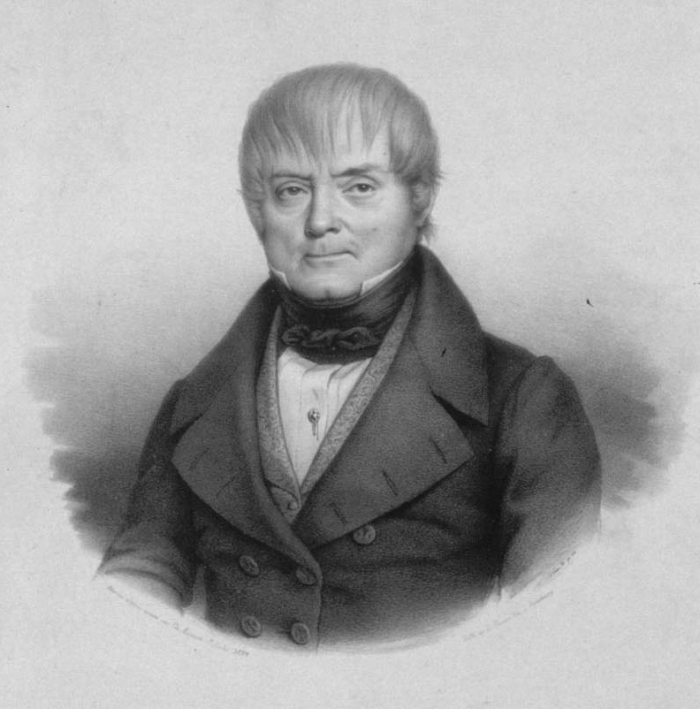
\includegraphics{shulmeister.png}

Человеческий ум чувствует склонность к контрастам, и это сказывается, между прочим, в том, что каждый продолжительный период мира влечет за собою подъем воинственного духа. Двадцать пять лет спустя после Ватерлоо останки Наполеона I торжественно переносятся с острова Св.Елены в дом Инвалидов. Седан и крушение второй империи навсегда, казалось, уничтожили обаяние рода Бонапартов; но вот появляются мемуары генерала Марбо и тотчас возникает увлечение императорскою эпопеею, а маршалы --- сподвижники Наполеона прославляются чуть не наравне с ним. История лишь выиграла от подобного возрождение прежней популярности: явились новые документальные данные, многие факты получили правдивое освещение, а деятельность многих сил --- более правильную оценку.

Однако ни в одном из новейших исследований мы не встречали имени человека, который, по свидетельству современных ему биографов и историков, уже с 1805 года приобрел большую известность и играл немаловажную роль в войне третьей коалиции. Этот человек --- Карл Шульмейстер, знаменитый шпион Наполеона I.

Такое умалчивание объясняется отчасти тем, что шпионств не принадлежит к числу правильно организованных средств разведывания, отчасти же тем, что, практикуемое в большинстве случаев людьми сомнительной нравственности и с корыстолюбивою целью, оно противно открытому и честному характеру французской нации.

И тем не менее судебные дела о шпионстве волнуют общественное мнение всех цивилизованных стран. Если человек молодой, сильный, блондин, с биноклем в руках, изберет местом своих прогулок какой-либо укрепленный район во Франции, он сильно рискует быть задержанным прохожими в качестве шпиона. Если незнакомец, брюнет коренастого сложения, займется фотографированием местности в Германии, его ожидает та же участь.

Но напрасно публика принимает так близко к сердцу подобные факты: шпионство, практикуемое теперь в мирное время, почти безвредно. В период французской революции и в первые годы империи военная география Европы была очень мало разработана: армии нуждались в хороших шпионах, хотя бы для заблаговременного ознакомления с дорогами. Теперь же топография не имеет секретов: железные, шоссейные, большие и малые грунтовые дороги, реки, каналы --- все это указано на прекрасных картах, которые всякий может приобрести; едва кончится возведение какого-нибудь форта, как он уже наносится на план; во французском Indicafeur Chaix отмечены все пути и линии, важные в коммерческом и стратегическом отношениях; немецкий Hendschel дает те же сведения относительно Германии.

В былые времена главнокомандующие армиями нуждались также в шпионах для получения сведений о производительности, богатстве неприятельского края и о численности соседних армий. Ныне статистика дает все нужные цифры: в Statistisches Jahrbuch fur das deutche Reich ежегодно помещаются данные о составе и распределении всех армейских корпусов; во Франции официальные документы столь же ясно обрисовывают положение дел. Стало быть в мирное время шпионство может иметь только две цели: или получение подробностей о постройке фортов, для чего нужен специалист, или присвоение мобилизационного плана. Последнее возможно только при условии подкупа чиновника или офицера, и вот почему закон так строго карает подобные преступления, составляющие государственную измену.

В военное время шпионство, как нам кажется, будет играть важную роль. Безусловно необходимо иметь сведения о положении неприятеля, о его силах и даже о его намерениях. Бесспорно, что эта задача должна быть выполнена кавалерией: но последняя может потерять соприкосновение с противником, как это случилось после Верта с немецкой армией, не знавшей о направлении движения Маг-Магона. Вообще в 1870 году сведения, получавшиеся немцами из побочных источников принесли им большую пользу. О сосредоточении армии Маг-Магона у Реймса и о предполагавшемся движении ее на соединение с Базеном главная немецкая квартира узнала из телеграммы посланной из Лондона. Таким же косвенным путем получено было немцами известие о движении французов для деблокады Бельфора. Следовательно, шпионы необходимы и не только на театре военных действий, но и во всей неприятельской стране. Очень часто подкуп неприятельского офицера дает громадные результаты. ``Если штабной офицер подкуплен за миллион, то это не дорого'',--- говорил принц де Линь.

Наполеон I прекрасно организовал шпионство и возложил высшее руководство им на генерала Савари, которому был подчинен и содействовал Шульмейстер. Он тратил громадные суммы и охотно прибегал к подкупу штабных офицеров, что не представляло особенных затруднений в ту эпоху, когда офицеры часто переходили на службу из одной армии в другую. Ниже упомянуто о нескольких австрийских офицерах, подкупленных Шульмейстером.

Самым громким делом Шульмейстера была капитуляция Макка. В течение нескольких лет после сдачи Ульма Шульмейстер считался одним из полезнейших сотрудников Наполеона; его открыто обвиняли в том, что, будучи взят Макком в качестве шпиона, он обманул австрийского главнокомандующего и много способствовал капитуляции Ульма. Это участие Шульмейстера в одном из важнейших событий первой Империи возбуждает особый интерес к основательному знакомству с деятельностью того человека, которого многие немецкие писатели называют ``злым гением Макка''.

\hypertarget{ux43bux435ux433ux435ux43dux434ux44b}{%
\chapter{Легенды}\label{ux43bux435ux433ux435ux43dux434ux44b}}

Немало анекдотов рассказывается о Шульмейстере, но достоверность их ничем не подтверждается. Одно из удивительнейших приключений Шульмейстера описано Каде-де-Гассикуром, лично знавшим его в 1809 году. Обыкновенно великий шпион, der grosse Spion, как называют его немцы, проникал на биваки или следовал за войсками, переодетый торговцем вина и табаку. В кампании 1805 года, в течение которой его присутствие удостоверено на очень значительном районе, он носил вероятно австрийский мундир, так как, будь он переодет разносчиком, вряд ли ему удалось бы вращаться свободно в армиях Макка и Кутузова и переезжать на громадные расстояния.

В Страсбурге до сих пор ходит рассказ о том, как Шульмейстер выбрался из осажденного города, лежа, как покойник, в гробу.

Однажды, как говорят, дом Шульмейстера был окружен австрийцами, он лично отпер дверь и свободно вышел на глазах солдат и жандармов, до того изменив свою наружность, что она совсем не соответствовала приметам указанным лицам, пришедшим арестовать его.

В сражении при Ваграме Шульмейстер едва не был взят в плен. Он бросился в соседний дом. Когда неприятельские солдаты вор-валиоь туда, по лестнице опускался цирюльник с мыльницей, кистью и всеми принадлежностями для бритья. То был Шульмейстер. ``Где шпион?'' --- спросили его солдаты,--- ``он укрылся в этом доме''.--- ``Поднимитесь на второй этаж; тяжело раненый, он лежит там на кровати'',--- отвечал Шульмейстер и быстро скрылся.

В Вене он также удачно избежал ареста. Когда подошли полицейские агенты, следившие за ним, он брился в парикмахерской; заметив опасность, Шульмейстер встал, вмиг вытер мыло с лица, дал золотой куаферу и убежал через задний ход. В Германии эта сцена была воспроизведена впоследствии на лубочной народной картине.

Выдавая себя за мелкого владетельного германского князя, он однажды произвел смотр неприятельскому армейскому корпусу и, благодаря этой хитрости, доставил ценные сведения французскому штабу.

В другой раз, переодетый австрийским генерал-интендантом, он присутствовал на военном совете, на котором председательствовал император Франц И. Шульмейстер заплатил миллион франков тому интенданту, имя и место которого он занял. Факт этот подтвердил нам один из наших приятелей Ипполит Пасси, участвовавший в последних кампаниях первой Империи и лично знавший Шульмейстера.

Некоторое время Шульмейстер ходил всюду с обыкновенной дворовой собачкой, на которой был постоянно надет чехол из кудрявой шерсти, превращавший ее в пуделя; под этим чехлом Шульмейстер прятал свои бумаги.

Отличительною его чертою была необыкновенная способность гримироваться. Достойный полной веры столетний старец рассказывал нам, что он часто видел Шульмейстера в 1830 году. Однажды, чтобы доказать ему свое искусство, Шульмейстер мгновенно преобразился: взбил рукою волосы, сделал одну --- две гримасы и стал совершенно другим человеком. Говорят, что в 1805 году он лично предложил свои услуги Наполеону. Он явился в Страсбурге в замок, в большом зале которого, на 1-м этаже, император принимал просителей. ``Какие у вас рекомендации?''--- спросил Наполеон.--- ``Никаких; я сам себя рекомендую''.--- ``В таком случае я не могу воспользоваться вашими услугами'',--- ответил император и отошел за ширму. Шульмейстер тотчас загримировался и изменил свою наружность до неузнаваемости. Думая, что он ушел, император вышел из-за ширмы и увидел перед собою незнакомца. ``Кто вы такой? Что вам нужно?''--- воскликнул изумленный Наполеон.--- ``Я Шульмейстер''. Пораженный такою ловкостью император тотчас принял его на службу.

По-видимому факты произошли иначе. Шульмейстер был вероятно рекомендован давно знавшим его генералом Савари, и, быть может, также Раппом. Некоторые биографы утверждают, что он был представлен первому консулу именно этими двумя генералами в 1804 году.

Все эти рассказы более или менее точны. Шульмейстер не любил, когда его называли шпионом, и под старость величал себя отставным военным наблюдателем и генеральным комиссаром армий. Достоверно только то, что щедро, по-императорски оплачивая труды его, Наполеон не дал ему ни одного ордена и даже резко отказал ему в этой просьбе. В минуты хорошего настроения духа император обращался очень фамильярно с прямыми своими подчиненными и любил говорить им ты. ``Шарль'',--- сказал он однажды Шульмейстеру, публично поблагодарив его за службу,--- ``ты один стоишь целой армии; проси чего хочешь: ни в чем не откажу''.--- ``Государь, прошу орден Почетного Легиона''.--- ``Денег, сколько хочешь'',--- ответил --- император,--- ``орден --- никогда; я берегу его для своих храбрецов''.

Трудно проследить исторический ход фактов, имеющих в основании полицейскую подкладку, ибо заслуга хорошей полиции заключается именно в том, чтобы действовать вполне секретно, не оставляя никаких следов. По отношению к Шульмейстеру дело усложняется еще тем, что он часто менял имя. Занимаясь шпионством в Ульме, в различных австрийских и русских корпусах, он называл себя то Шульмейстером, то Бургермейстером. При официальных поручениях, которые давались ему в Вейсмаре и Кенигсберге, его называли Шарлем или де-Шарль; в своих поместьях он становился господином де-Мейнау. В небольшой анонимной брошюре, изданной в защиту Шульмейстера в Лейпциге в 1817 году, говорится, что в большинстве случаев он отказывался от своей настоящей фамилии ввиду трудности произношения ее для французов. И действительно имя Шульмейстер, произносимое по-немецки Шульмайстр, сильно коверкалось французами, которые не могут правильно выговорить даже такие названия как Кобленц, Кельн, Майнц и Мюнхен. Каде-де-Гассикур, например, пишет Шульместер. Нет ничего удивителвного в том, что Шульмейстер, богатый помещик, владелец отеля в Париже, одного замка в Эльзасе, другого --- тоже в Париже, человек запросто знакомый с генералами и министрами, герцогами и графами, стал величать себя де-Мейнау.

Один из немецких ученых, Фердинанд Диффенбах, посвятивший биографии Шульмейстера брошюру в сотню страниц\footnote{Karl Ludwig Schulmeister, der Hauptspion, Parteiganger Polizeprafect und geheime Agent Napoleon I - Лейпциг, издание I. Н.Вебеля. 1879. Брошюра in---8°,96 с}, наводил справки в архивах военного министерства в Вене и Берлине и внутренних дел в Берлине, в городских архивах Вены, Кенигсберга, Страсбурга, Штетина, Вейсмара, в бюро записей и в городской библиотеке Страсбурга, наконец, в делах Ней-Фрейштадтской коммуны. Он добыл все, что есть официального в Германии, и подробно изучил этот материал. Мы почерпнули многое из указанного труда.

В свою очередь мы справлялись во французских военном и национальном архивах и нашли там в документах, относящихся к 1805, 1806, 1807, 1808 и 1809 гг., рапорты, составленные Шульмейстером, и различные касающиеся его бумаги; ниже помещаем большинство из них.

Заслуживает также внимания брошюра, изданная в 1817 году в Лейпциге\footnote{Brüchstucke aus dem Leben des Charles Shulmeister von Meinau als anderklagter Hauptspion des Napoleon - Лейпциг. 1817. in---18, 104c}. Анонимный автор ее, выставляя себя приверженцем правдивости, говорит, что она составлена со слов прусского чиновника, отвозившего Шульмейстера в 1815 году из Парижа в крепость Везель и очень полюбившего его. Она написана если не самим Шульмейстером, то во всяком случае по его личным указаниям. В ней изложена масса фактов, но есть также много предумышленных ошибок. Подвергнутый тюремному заключению в 1815 году, Шульмейстер опасался вторичного арестования, во избежание чего подтасовывал факты. В брошюре рассказана история семьи Шульмейстера.

\hypertarget{ux43fux435ux440ux432ux430ux44f-ux434ux435ux44fux442ux435ux43bux44cux43dux43eux441ux442ux44c-ux448ux443ux43bux44cux43cux435ux439ux441ux442ux435ux440ux430}{%
\chapter{Первая деятельность Шульмейстера}\label{ux43fux435ux440ux432ux430ux44f-ux434ux435ux44fux442ux435ux43bux44cux43dux43eux441ux442ux44c-ux448ux443ux43bux44cux43cux435ux439ux441ux442ux435ux440ux430}}

Как большинство авантюристов, Шульмейстер утверждает, что он происходит из знатного рода. По словам Brüchtucke, в 1730 году в Эльзас прибыл венгерский дворянин Берский, вынужденный бежать из отечества вследствие дуэли, кончившейся смертью его противника. Берский поселился в графстве Ганау-Лихтенберг, которое состояло из 14 городов и 160 деревень с населением в 100.000 чел.; в состав его входили: в Эльзасе --- теперешний кантон Буксвейлер и часть кантонов Гохфельден, Нидербронн, Верт, Бру-мат; в Пфальце --- округ Лембах; в великом герцогстве Баденском --- округа Вильштет и Лихтенау. Эльзасская часть графства находилась в подчинении Франции, а другая половина зависела от священной Римской империи. Берский нашел приют у сельского учителя (Schulmeister), занял место его помощника и тем охотнее стал называться Шульмейстером, что обстоятельства вынуждали его скрывать свою настоящую фамилию.

Граф Жан-Рене Ганау назначил преемником своим в графстве своего внука Людовика IX, старшего сына ландграфа Людовика VIII Гессен-Дармштадтского и наследницы Ганау. С 1735 года Людовик IX жил в Буксвейлере, а в 1741 году, по достижении совершеннолетия, принял в свои руки бразды правления. Он знал Берского, уважал его и назначил, под фамилиею Шульмейстера, окружным приставом в Лихтенау.

Весьма вероятно, что рассказ о происхождении Верского --- плод богатой на выдумки фантазии наполеоновского шпиона. Трудно допустить, чтобы в эпоху, когда выдача преступников была обставлена очень большими затруднениями, венгерский офицер укрылся в маленькой сельской школе и даже не попытался поступить на жалование в какую-нибудь армию.

Тем не менее в приходских церковных книгах значится окружной пристав Христиан-Годфруа Шульмейстер, который был женат, слыл за хорошего мужа и отца и умер безбедным. Его сын Жан-Годфруа изучал теологию, был пастором в Лейтесгейме, а в 1763 году --- в Ней-Фрейштадте, верстах в двадцати пяти от Страсбурга, на правом берегу Рейна.

У пастора было три сына: Жан-Годфруа, черепичник в Бадерсвейере, Шарль-Луи, наш герой, и еще один, умерший пастором в Ней-Фрейштадте в 1833 году. Метрическое свидетельство второго сына найдено Диффенбахом в церковных книгах; оно составлено самим отцом.

Карл Шульмейстер родился 5 августа 1770 года, крещен 8 августа; крестными отцами его были лейтесгеймский пастор и казначей бишофсгеймской фабрики; крестного матерью --- жена пастора Легельсгурста. Шульмейстер получил очень хорошее по тем временам воспитание и образование, что доказывают рапорты составленные им впоследствии при исполнении военных поручений. Он женился рано, 20 февраля 1792 года, на дочери бурграта Унгера, в Сент-Мари-о-Мин; ему было тогда 22 года, жене --- 18 лет. В делах гражданского управления С.-Мари сохранился брачный акт. Шульмейстер подписался ``Шарль-Луи Шульмейстер'' в должности актуариуса (секретаря) канцелярии княжества Дармштадтского в Корке, селении на правом берегу Рейна, в 10 верстах от Страсбурга. Шафером и свидетелем с его стороны был его родной брат Жан-Годфруа. Брачные акты составлялись на немецком языке в Сент-Мари-о-Мин (Маркирх) и носили довольно странное название Copulations-Buch der Evangelisch-Lutherischen gemeinde, т.е. Peeстр брачных соитий евангелическо-лютеранского прихода.

В 1797 году Шульмейстер был в своем родном селении торговцем железными изделиями; при переписи 1798 года он записан как негоциант, проживающий в Страсбурге с 1797 года. Его отец умер в 1793 году. Находя контрабанду весьма выгодной, сын сделался контрабандистом; молодой и смелый, он лично провозил товары Тому назад лет 25 или 30 в Ней-Фрейштадте проживали еще старики, помнившие его проделки на Рейне. Застигнутый однажды пограничным стражником в ту минуту, как он причаливал к левому берегу, Шульмейстер убил его выстрелом из пистолета; факт этот неоднократно подтверждался. Действуя один, Шульмейстер не мог иметь большой денежной прибыли, поэтому он вербовал контра бандистов, которые работали на него.

Шульмейстер не отрицает этих фактов: в Brüchstucke сказано, что контрабанда служила ему золотым дном. Но он уверяет, что занимался этим ремеслом лишь с 1800 по 1805 год; что, поступив 17-ти лет от роду во французский гусарский полк, он участвовал почти во всех революционных войнах и, в особенности, в кампании Моро, а в 1800 году вышел в отставку с чином adjudant-commandant. Невероятность продолжительной службы Шульмейстера в рядах армии бросается в глаза. Можно ли допустить, чтобы тридцатилетний полковник вышел в отставку ради контрабандной торговли? Это опровергается бесспорными официальными данными: с 1792 по 1797 год Шульмейстер записан торговцем железными изделиями в своем родном селе, а с 1798 по 1805 год --- торговцем колониальными товарами и табаком в Страсбурге. В течение этого продолжительного периода он занимался контрабандой, чему благоприятствовало течение Рейна и его многочисленные острова; до 1860 года подобное ремесло было очень прибыльно и практиковалось многими баденцами и эльзасцами. Вероятно Шульмейстер продолжал заниматься им и в последние годы Империи при содействии или, по меньшей мере, при попустительстве чиновных лиц, умышленно закрывавших глаза на проступки слуги Наполеона I.

Занимаясь контрабандой, Шульмейстер не упускал случая заработать деньги иными путями. Он утверждает, что находился в рядах армии Моро и там сошелся с Савари. Моро переправлялся через Рейн в IV, V и VIII годах, каждый раз близ Ней-Фрейштадта, где проживал Шульмейстер до 1797 года. Савари принимал участие в этих трех кампаниях; во главе пехотного батальона он первый переходил через реку как в IV, так и в V году.

По всей вероятности Шульмейстер был мелочным торговцем, каких много в хвосте каждой армии; он продавал солдатам водку и табак и был замечен генералом Савари, воспользовавшимся его услугами. В своем рапорте от 26 октября 1805 года, Шульмейстер упоминает об австрийском офицере Рульцком, своем пособнике, с которым он сошелся во время последней войны. Следовательно, уже в 1800 году он несомненно занимался шпионством.

Диффенбах полагает, что Шульмейстер служил также в тайной (сыскной) полиции. Страсбургский префект установил секретный надзор за эмигрантами, проживавшими в большом числе на правом берегу Рейна, в Оффенбурге, Эттенгейме, Фрейбурге; префект собирал сведения и с более удаленных немецких владений.

Драке и Спенсер Смитт, представители Англии, первый в Мюнхене, второй в Штутгарте, руководили заговорами против Франции; им помогал их коллега в Швейцарии, Виккам. В конце сентября 1803 года в Келе был задержан французский заговорщик Меге-де-Леклюз, посланный Драке в Париж. Чтобы избавиться от смерти, Леклюз изменил Драке и перешел на службу во французскую полицию. Через посредство капитана Розей, носившего звание адъютанта заговора, Леклюз отправил Драке письма, написанные под диктовку префекта Нижнего Рейна, Зее. Розей ездил два раза в Мюнхен и Штутгарт, получил от Драке и Спенсера Смитта 130.000 франков и передал их префекту Зее. Таким путем правительство первого консула добыло все документы, относившиеся до происков английских уполномоченных. Мы приводим этот факт главным образом в виду поведения Розей. Если капитан позволял себе подобные поступки, то неудивительно, что Шульмейстер, агент Наполеона, предложил свои услуги Макку в качестве шпиона; а так как у контрабандиста совесть более покладиста, чем у воина, то он и оставил в свою пользу деньги Макка и Мерфельдта. Но не будем забегать вперед.

Особенный надзор был установлен за герцогом Энгиенским, который проживал в Эттенгейме. Герцог вел себя неосторожно и некоторое время приезжал еженедельно на спектакль в Страсбург. Диффенбах полагает, что надзор за Эттенгеймом был возложен на Шульмейстера, который, благодаря занятию торговлею, мог появляться всюду и, живя в Страсбурге, часто приходит под предлогом торговых дел в близлежащий Эттенгейм. Нугаред де-Файе\footnote{Recherches historiques sur le proces de due d'Enghien. Париж, 1844 г} ссылается на письмо нижнерейнского префекта к министру юстиции от 17-го вентоза (шестой месяц республиканского года) XII года, в котором упоминается о письменной справке по этому делу, наведенной гражданином S \ldots{} (Фамилия вычеркнута) .

Но мнение Диффенбаха ошибочно. Одновременно с задержанием герцога Энгиенского был арестован маркиз Тюмери, которого приняли за Дюмурье. Отлично владевший французским языком, Шульмейстер не смешал бы Дюмурье с Тюмери. Кроме того в сентябре 1805 года по распоряжению префекта Шульмейстер был выслан из нижнерейнского департамента, что бесспорно явствует из его рапорта № 2 от 21 октября 1805 года и из официальной бумаги от 18 марта 1806 года\footnote{см. страницы 51-ю и 68-ю}. Мог ли Зее подписать постановление о высылке человека, услугами которого он пользовался в деле Розей и при надзоре за герцогом Энгиенским. Разумеется, нет.

Рассказы Шульмейстера о своей деятельности до 1805 года опровергаются фактами. Он говорит в Brüchtucke, что, находясь в отставке, занимался покупкою и продажею недвижимых имуществ, земледелием и, в особенности, контрабандой, заработав при этом крупный капитал. Диффенбах подробно рассмотрел страсбургский архив и в результате выяснилось, что с 1797 по 1805 год Шульмейстер был записан сначала как мелочной бакалейный торговец, затем как табачный фабрикант и владелец лишь одного незначительного недвижимого имущества; он разбогател только с 1806 года.

Шульмейстер рассказывает далее, что его коммерческое благосостояние возбудило против него власти, что его арестовали, продержали в заключении в Страсбурге два месяца и выпустили на свободу по неимению улик. Немного спустя он был вторично задержан и препровожден за границу с воспрещением возвращения на французскую территорию. Он поселился в Бадене. Вскоре возгорелась война. Вооруженный против Наполеона, Шульмейстер предложил свои услуги Макку, был зачислен в австрийский штаб, ревностно служил союзникам, но был заподозрен и арестован. Оставшись на свободе при отступлении австрийцев, он просил покровительства у своего бывшего сослуживца Савари, который назначил его комиссаром в Вене, после чего Шульмейстер почти поневоле оставался на службе во французской полиции до 1810 года.

Таков рассказ самого Шульмейстера. В 1817 году, когда издана была его книга, он опасался нового арестования союзниками, которым реставрация не отказала бы в выдаче бывшего шпиона Наполеона I, обвинявшегося в содействии возвращению императора с острова Эльбы. Шульмейстер стремился обелить себя. Он выставлял себя баденцом, верно служившим сначала Австрии, а затем Франции. Следовательно, его не могли бы обвинить по делу о капитуляции Макка. Но найденные нами в Париже ниже помещенные документы доказывают, что все утверждения Шульмейстера вымышлены и что с самого начала кампании 1805 года он работал для французской главной квартиры.

\hypertarget{ux443ux43bux44cux43c}{%
\chapter{Ульм}\label{ux443ux43bux44cux43c}}

Третья коалиция составилась в апреле 1805 года; договор между Англией и Россией был подписан 11 апреля, но Австрия примкнула к коалиции лишь 11 августа и то скрывала этот факт в течение нескольких дней.

Вынужденный в конце августа отказаться от высадки в Англию вследствие неопытности Вильнева, Наполеон решил перенести войну в Германию. Противник же ожидал наступления французов со стороны Италии, а не Германии, и потому сосредоточил главные силы на юге.

40.000 человек, под начальством эрцгерцога Иоанна должны были действовать в Тироле, а 100.000, под начальством эрцгерцога Карла, сосредоточились на Адиже. В Германии Австрия была в состоянии выставить только около 60.000 человек. Две русские армии, собиравшиеся в Галиции и в Польше, могли присоединиться к австрийским войскам лишь после месячного похода.

Владея переправами на Рейне и имея 200.000 человек, Наполеон легко мог атаковать австрийцев до их соединения с русскими. Насколько можно было, император откладывал свой отъезд из Булони и вместе с тем послал Мюрата в Баварию под вымышленным именем для рекогносцировки путей от Рейна к Дунаю; такие же поручения возложены были на Савари и Бертрана. Благодаря многочисленным агентам Наполеон точно знал ежедневные передвижения каждого австрийского полка.

Затем Мюрат расположился в Страсбурге, где оставался до 29 сентября, и в этот день перешел Рейн у Келя. К нему приезжала масса курьеров от французских уполномоченных из Штутгарта, Регенсбурга и Мюнхена; он же доносил обо всем императору. В архиве военного министерства сохранилось много донесений: его, генерала Бертрана и префекта Зее.

Австрийской армией номинально начальствовал эрцгерцог Фердинанд, в действительности же генерал Макк. 16 августа она начала наступление и к 7 сентября заняла Баварию. Курфюрст Баварский со своими 25.000 человек отступил в Вюрцбург. Следуя за ним, Макк занял Ульм, у которого в 1800 году Край задержал Моро; австрийцы расположились вдоль Иллера, от Кемптена до Ульма, ожидая дебуширования французов из Шварцвальдских проходов; правое крыло протянулось по Дунаю до Гюнцбурга. Связь между Макком и Австрией поддерживал Кинмайер, занимавший Нейбург, Ингольштадт, Эйхштадт, Эльванген и Амберг.

В это время Наполеон направлял Великую армию к Рейну, соблюдая возможно большую тайну; он распускал слух, что двигает только 30.000 человек для наблюдения за австрийцами. Министру полиции император писал: ``Запретите газетам говорить об армии, как будто ее в действительности вовсе не существует''. Между тем к Рейну и Дунаю наступали семь корпусов.

Мармон шел вверх по Рейну из Голландии до Майнца, откуда свернул на Вюрцбург для соединения с Бернадоттом, следовавшим из Гановера под предлогом возвращения во Францию. Соединение состоялось 29 сентября.

Корпуса Даву, Сульта, Ланна, Нея и Ожеро к 24 и 25 сентября с берегов океана были переброшены на Рейн и сосредоточились в Мангейме, Шпейере и Майнце; союзники не имели ни малейших сведений о движении этой массы людей.

Император лично оставался в Булони до 2 сентября; чтобы еще лучше скрыть свои операции, он провел затем три недели в Сен-Клу, откуда выехал 24-го, прибыл 26-го в Страсбург, где по-видимому занимался только устройством празднеств, а 1 октября перешел Рейн. Узнав о расположении Макка под Ульмом, он решил не разбить Макка, чтобы затем обратиться против русской армии, а совершенно уничтожить его, т.е. обойти и окружить. Мюрату с кавалерией было послано приказание занять австрийцев демонстрацией с фронта, наступая как бы в голове армии через Вальд-д'Анфер. Во исполнение этого 29 сентября кавалерия переправилась через Рейн у Келя.

Тем временем обходное движение французской армии совершалось по трем путям: Наполеон с корпусами Ланна, Нея и с гвардией шел через Пфорцгейм, Штутгарт и Гейденгейм; корпус Сульта --- через Гейльброн, Эльванген и Нордлинген; корпус Даву --- через Гайдельберг, Ингельфинген и Этинген. Вся армия должна была стать 7 октября за Макком на Дунае, от Донауверта до Инголь-штадта. 4 октября Мюрат был отозван с кавалерией из шварцвальдских проходов и быстро присоединился к Наполеону.

Демонстрации Мюрата и донесения шпионов окончательно ввели Макка в заблуждение; он ждал французов с фронта, а войска, движение которых было обнаружено на севере, принимал за небольшое подкрепление, высланное баварцами в Вюрцбург.

Предначертанный Наполеоном марш французской армии был выполнен в точности. Кинмайер отступил вскоре на Мюнхен. В это время Макк мог еще отойти с Иллера на Лех и присоединиться к Кинмайеру через Аугсбург на мюнхенской дороге; но он упорствовал в своем первоначальном решении.

9 октября дивизия Удино, корпуса Ланна, овладела Вертингеном к югу от Дуная, в 24 верстах от Донауверта. В тот же день Ней взял с бою Гюнцбург и бывший там мост. Правое крыло Макка отступило к Ульму.

Переправившись через Дунай у Инголынтадта, 10-го Бернадотт овладел Фрейсингеном, так что Кинмайер оказался совершенно отрезанным от Макка и отступил к Инну. Движение австрийцев от Гюнцбурга к Ульму доказывало, что Макк не думал о прикрытии своих сообщений с Кинмайером и с ожидавшеюся русской армией. Поэтому Наполеон поспешил завершить окружение Макка.

Вскоре все пути от Ульма в Австрию оказались в руках французов. Наполеон с гвардией и корпусом Мармона стоял в Аугсбурге; Даву и Бернадотт --- в Дахау и Мюнхене; Ней овладел Альбеком и Эльхингеном на левом берегу Дуная и связывался с правым берегом через посредство Ланна и Мюрата, расположенных от Лейпгейма до Бургау.

Макк мог еще отступить левым берегом, где корпус Нея был слишком слаб для его удержания, и достигнуть или Богемии через Аален и Нордлинген, или Тироля через Мемминген. Наполеон полагал, что Макк предпочтет отступление на юг. Поэтому 11-го числа Сульт выступил из Аугсбурга к Меммингену, где Шпанген поддерживал сообщение с Тиролем. По распоряжению Мюрата Ней переправил дивизии Дюпона и Бараге-д'Иллье на правый берег и двинул их к Иллеру, вдоль которого, по предположениям французов, следовал Макк направляясь на юг. Дюпон не мог исполнить данного ему предписания, потому что столкнулся с австрийцами у Гаслаха и должен был отступить к Лангенау. Макк принял отступление Дюпона за поражение и еще более уверился в наступлении главных сил противника с запада.

11 -го числа французские дивизии достигли Вейссенгорна и Ил-лертиссена, приблизительно в 24 верстах от Ульма. Макк бросался от одного предположения к другому. 13-го он, по-видимому, намеревался пробиться по левому берегу к Гендейгейму. В это время получено было сведение о появлении французского корпуса на Иллере. По словам Диффенбаха это известие было передано Макку Шульмейстером. Вместе с тем распространился слух о высадке англичан в Булони и о контрреволюции в Париже.

Бедный Макк сейчас же вообразил, что обнаруженное на Иллере движение французов было началом их отступления к Рейну. Он тот час принял соответственные меры: Иелачич должен был оставаться в стороне Меммингина для преследования французов, отступающих к Шварцвальду; Ришу приказано двинуться к Инну для встречи русских; Вернеку --- оставаться на севере до Аалена. 14-го утром Макк издал приказ о преследовании французской армии; по его предположениям она состояла из трех корпусов отходивших: первый --- через Мемминген, второй --- через Иллертиссен, третий --- через Донауверт. Соответственно этому даны были распоряжения Иелачичу, Шварценбергу, Вернеку и Ришу. В военной истории не подберешь второго примера подобной бессмыслицы и подобных предвзятых идей.

Еще после полудня 14-го числа Макк объявил эрцгерцогу Фердинанду, что 15-го Дунай и Иллер будут очищенны французами и путь на Аугсбург окажется свободным.

14-го вечером он вторично подтвердил Варнеку приказание преследовать неприятеля совместно с Шварценбергом.

Между тем 14-го Сульт бомбардировал Мемминген и к вечеру Шпанген сдал город. Иелачичу, которому предписывалось преследовать отступавших в этом направлении французов, пришлось целый день обороняться против Сульта; ему удалось уйти через Лейткирх на Вангер и 16-го достигнуть Форарльберга.

В тот же день, т.е. 14-го числа, Мармон и Ланн заняли Обер и Нидер-Кирхберг и Геклинген; таким образом было закончено обложение Ульма с правого берега Дуная. На левом берегу Дюпон взял Альбек. Ней покрыл себя славой у Эльхингена: овладев Эльхингенским монастырем и мостом, он обеспечивал сообщение между двумя берегами; войска Риша были оттеснены им в Юнгинген под стенами Ульма.

К вечеру закончилось обложение Ульма со всех сторон. Правильно оценивая обстановку, с наступлением сумерек эрцгерцог Фердинанд выступил из Ульма во главе 2.000 человек и спасся через Гейслинген. Макк же не переставал уверять его, что французская армия находится в отчаянном положении и боем лишь прикрывает свое отступление. В тот же день Макк отправил Шульмейстера, который в официальной записке назван его доверенным шпионом, в Штутгарт, чтобы навести справки о высадке англичан и о парижской контрреволюции.

По мнению генерала барона Тьебо Макк мог еще после потери Меммингена отойти на юг. Дело в том, что Сульт двинулся на Биберах без предварительной рекогносцировки дороги, которая на протяжении около 12 верст идет в выемке и крайне неудобна для движения войск. Следовавшая в голове колонны артиллерия застряла. Настала ночь, и в войсках, только что одержавших победу, произошел полнейший беспорядок. Если бы Макк подошел в это время, то застал бы корпус Сульта в таком расстройстве, что без труда раздавил бы его. Таков взгляд, изложенный в мемуарах Тьебо; но надо заметить, что автор их был всегда самым ярым критиком Сульта.

15-го Макк издал приказ, перевод которого на французский язык сохранился в архиве французского военного министерства: ``Через несколько дней, говорит он, авангарды двух могущественных армий, австрийской и русской, явятся нам на выручку. Неприятельская армия находится в самом плачевном положении, как вследствие дурной погоды, так и вследствие недостатка жизненных припасов; она не в состоянии больше держаться на занятых местах, штурм же может вестись лишь незначительными частями; а так как мы окружены широкими водяными рвами, то уничтожение или пленение неприятеля не представляет никаких затруднений''.

В тот же день Ней взял с бою Михельсберг, командующий над всем городом. Дальнейшая оборона крепости становилась невозможною. Вернек был отрезан от Ульма и направился в Богемию; с ним соединился Фердинанд. Преследование этих отрядов было возложено на Мюрата. Ней приступил к бомбардировке Ульма, и Наполеон предложил Макку сдаться.

16-го утром Макк изъявил согласие на сдачу крепости, причем переговоры велись через Лихтенштейна, который был принят императором. Затем Макк подтвердил письменно свое согласие, обещая отдать крепость в тот же день, а войска вывести 18-го числа, с тем однако, чтобы им разрешено было уйти в Австрию.

В ночь с 16-го на 17-е к Макку был отправлен Ф.де-Сепор; в своих мемуарах он дал очень живое описание переговоров с австрийским фельдмаршалом.

Бертье и Макк подписали договор, в силу которого 18-го числа одна французская бригада заняла крепость; австрийский гарнизон должен был оставаться там до 12 часов ночи 25-го числа и, если бы к этому сроку на выручку ему не явилась другая австрийская армия, он считался бы военнопленным и подлежал отправлению во Францию; офицеры получили свободу под честным словом.

19-го Наполеон пригласил Макка в Эльхивген и сообщил ему о сдаче Мюрату корпуса Вернека 18-го числа. Окончательно упавши духом, Макк согласился на сдачу армии 20-го в 3 часа вечера, под условием, что корпус Нея останется в Ульме до 25-го.

20-го плененная армия продефилировала перед императором. Согласно дневного приказа по армии, составленного в Эльхингене 20 октября, Макк сдал в Ульме 25.000 чел., 8 генералов, 50 запряженных орудий, 3.000 лошадей и 40 знамен. В Меммингене взято 5.000 человек, в Эльхингене --- 3.000, в других делах -6.000 чел. и 2.000 лошадей. 20.000 чел. под начальством Иелачича, Кинмайера и Фердинанда успели спастись.

Таковы факты. Ф.де Сегюр прекрасно обрисовал жалкую личность, которой Австрия вверила свою армию. Немецкие историки характеризуют его как пустослова и педанта, способного только на управление каким-нибудь министерским бюро. Ему не следовало доверяться, так как уже в Неаполитанском королевстве он завязывал переговоры с французскими генералами; обвиненный своими подчиненными, он бежал к Шампионе. Еще раньше, в чине полковника и в должности начальника штаба принца Саксен-Кобурского, он принимал участие в переговорах с Дюмурье. В активе у него значилась лишь одна победа при Альденговене, одержанная эрцгерцогом Карлом, у которого он был начальником штаба. После сражения муниципалитет поднес эрцгерцогу лавровый венок, а тот любезно отдал половину венка Макку. С этого дня Макк уверовал в свое важное значение и стал заказывать портреты и медали, на которых он изображался с лавровым венком на каске.

Макк составил два мемуара: один был подан им военному суду, которому он был предан, и составляет библиографическую редкость; другой представлен императору Францу II уже после произнесения приговора и отпечатан впервые в 1873 году в Лейпциге фирмою Брокгауза в Historisches Taschenbuch: в нем Макк пытается опровергнуть по пунктам весь обвинительный акт. Оба мемура наглядно доказывают тщеславие и неспособность фельдмаршала.

Какую роль играл во всем этом событии Шульмейстер? Французские и немецкие историки единогласно свидетельствуют, что при Макке состояло несколько французских шпионов. Прибегая к их услугам, император лишь следовал прежней прекрасной системе и как итальянец был верен своему природному инстинкту к лукавству. Баррас\footnote{Memoires, том П, стр. 108} утверждает, что тотчас по прибытии в Италию в 1796 году Бонапарт организовал тайную полицию и следил за Людовиком XVIII, ни на минуту не теряя из виду всех Бурбонов. Сегюр\footnote{Histore et Memoires, том II, стр. 54} рассказывает, что после перехода через С.-Бернар Наполеону явился один из шпионов, отлично служивший ему в 1797 году. ``Как! - Воскликнул первый консул, - тебя еще не расстреляли?'' Шпион ответил, что после отъезда Бонапарта в Египет он перешел на сторону неприятеля, но теперь решил вновь связать свое счастье со счастьем Бонапарта и за 24.000 франков берется ввести неприятеля в заблуждение ложными донесениями, которые ему продиктует первый консул. Было заключено условие, шпион исполнил свое обешание, и Бонапарт считал описанную встречу милостью фортуны.

Тьер упоминает о ложных донесениях, ловко переданных Маку Наполеоном через посредство шпионов.

По словам Бюлова\footnote{Der Feldzug von 1805, изд. в 1806 году} 13-го числа Макк был убежден, что 14-го французы отступят, и еще более уверился в том из донесения шпиона, которого считал преданным австрийскому делу, между тем как в действительности он был подослан Наполеоном.

Моригль\footnote{Der Feldzug von 1805, Инсбрук, 1861 г} уверяет, что обманутый шпионами Макк был убежден, что французы отступят все до последнего 14-го числа; в числе двойных шпионов Моригль называет Шульмейстера.

Людвиг Гейссер рассказывает в Deutsche Geschichte, что Наполеон отправил к Макку известного двойного шпиона Шульмейстера, который объявил ему о контрреволюции в Париже, о высадке англичан и об отступлении Наполеона.

Диффенбах посвящает длинную главу роли Шульмейстера в Ульме: но так как он основывается только на немецких документах, то и не может доискаться истины.

Доктор Август Фурнье, профессор Пражского университета, утверждает в не так давно опубликованном труде \footnote{Napoleon I-er, изд. Фрейтага, Лейпциг, 1888 г}, что двойной шпион Шульмейстер доставлял Макку точные сведения о передвижениях французских корпусов; но твердо уверенный, как и все высшие сановники в Вене, что трон Наполеона покоится на зыбком основании, австрийский фельдмаршал смотрел на эти передвижения, как на отступление к Рейну, вынужденное парижскою контрреволюцией; Шульмейстер же убедился, что дело окончательно проиграно Австрией лишь тогда, когда Макк послал его за получением сведений в Штутгарт, после чего он и сделался верным слугою Наполеона.

Дознание, произведенное по повелению австрийского правительства, выяснило, что Макк неоднократно беседовал с Шульмейстером. Сначала Макк отрицал это; он признался уже позже и показал, что выдал Шульмейстеру паспорт и послал его в Штутгарт, чтобы выяснить, отступают ли французы; но Шульмейстер не вернулся. Макк показал также, что Шульмейстер имел смелость просить у него в присутствии генерала Кленау дутый или истинный списочный состав армии и что он хвастал, будто подкупил комиссариатского чиновника французской главной квартиры.

Но дознанием выяснилось также, что 13-го числа Шульмейстер объявил Макку в присутствии Шварценберга и Гиулая о движении французов на Мемминген, причем прибавил, что план Наполеона заключался в пресечении сообщений австрийцев с Тиролем, в движении с остальною частью армии на Эльхинген и Альбек и в овладении Ульмскими высотами: события доказали верность донесений Шульмейстера.

При дознании граф Мерфельдт показал, что Шульмейстер, услугами которого неоднократно пользовались Макк и эрцгерцог Фердинанд, являлся к нему с паспортом подписанным Макком, в Бранау, где находился штаб Мерфельдта с 18-го по 26 октября, доставлял ему важные и верные сведения, знал точно передвижения французских корпусов и несомненно имел доступ во все штабы, чем не мало гордился. Граф Мерфельдт дал ему 100 дукатов и паспорт. Шульмейстер обещал вернуться, но больше не показывался.

В Bruchstucke рассказывается приблизительно то же самое. По помещенным там сведениям, в октябре 1805 года Шульмейстер выказал себя верным агентом Австрии.

Как же примирить результаты дознания с общераспространенным мнением о роли Шульмейстера? Рассмотрение защиты Макка указывает путь для разрешения этого вопроса, а ознакомление с перепиской, которая велась во французской армии, приводит к выяснению истины.

Согласно обвинительному акту Макк был виновен в том, что:\\
1) поверил ложному известию о высадке англичан в Булони и о революции во Франции;\\
2) принял движение французской армии к Иллеру за отступление;\\
3) не слушал предостережений одного из лучших своих шпионов, который сообщил ему о намерении Наполеона отрезать австрийцев от Тироля и окружить их в Ульме, и который добровольно вызывался быть заложником в удостоверение правдивости своих показаний.\\
Шпионом этим был Шульмейстер.

Макк возражает в своем мемуаре, что Шульмейстера напрасно считали одним из лучших его шпионов, что он, Макк, не доверял ему, так как однажды Шульмейстер выпрашивал у него списочное состояние армии, что может подтвердить фельдмаршал-лейтенант Кленау. Макк прибавляет, что этот шпион в отношении своей нравственности ничем себя не зарекомендовал, ибо служил только за деньги, не был даже подданным его величества императора австрийского; его же предложение остаться заложником не имело никакого значения, ибо он мог всегда сказать, что неприятель изменил свой первоначальный план, причем знал отлично, что за это его не повесят.

По словам Макка, тотчас по приезде в армию эрцгерцог Фердинанд поставил во главе разведочной части путем шпионства некоего Венда, рекомендованного ему военным министром, дав ему чин и содержание капитана. Никто не знал прошлого Венда. Этот капитан бесконтрольно распоряжался разведками, получал необходимые суммы и посылал донесения эрцгерцогу и Макку. Следовательно, лучший шпион был у Венда, а не у главнокомандующего. По мнению Макка, обвинительный акт несправедливо возлагает на главнокомандующего ответственность за выбор шпионов, которая всецело падает на капитана заведывавшего разведывательною частью. Между тем 15 октября утром в своем рапорте, последнем до периода полного обложения, Венд не говорит ни слова о предстоявшей в тот же день блокаде, а наоборот, утверждает, что Геклингенский мост возобновлен ночью и что неприятель очевидно намеревается отступить по этому мосту на Блауберен. Итак, до последней минуты Венд подкреплял убеждение главнокомандующего, так как Блауберен находится в трех милях западнее Ульма, на дороге из Ульма через Урах в Штутгарт.

В рапорте от 21 октября, посланном Савари, Шульмейстер доносит, что, вернувшись в Ульм 19-го числа, он имел продолжительное свидание с Вендом, причем дает точные подробности об операциях австрийской армии, сообщенные ему Вендом; в рапорте от 26-го октября, адресованном также Савари, он указывает положение армий Кинмайера и Кутузова, основываясь на осмотре их, произведенном совместно с капитаном Вендом и Рульцким. Благодаря этим двум рапортам, хранящимся в переписке Великой армии, легко выяснить роль Шульмейстера.

После постановления нижнерейнского префекта о высылке Шульмейстер отправился в Германию; в австрийской армии он встретил своего приятеля капитана Рульцкого и капитана Венда, стоявшего во главе разведочной части; Шульмейстер вступил с ними в переговоры и, заручившись их содействием, тайно вернулся в Страсбург; здесь благодаря Савари он был представлен императору и заключил с ним условие подобно тому шпиону, о котором говорит Сепор в своем труде.

Впоследствии в своих разговорах с почтенными жителями Страсбурга, показания которых были собраны Диффенбахом и заслуживают полной веры, Шульмейстер сознавался, что 1 октября в Страсбурге получил аудиенцию от Наполеона. Он был подчинен адъютанту императора, Савари, который заведывал шпионством и полицией. Шапталь\footnote{Souvenirs sur Napoleon, стр. 381} упоминает о полицейской роли адъютантов и генералов императорской свиты. Госпожа де Ремюза \footnote{Memoires, том II, стр. 246} рассказывает, что на время этой кампании Савари получил большой ящик с золотом для уплаты жалования полицейским агентам в армии и в завоеванных городах, причем он действовал очень ловко и знал буквально все.

Мемуары Фуше, изданные в 1824 году, также упоминают о роли Шульмейстера. Правда, против изложенного в Мемуарах, тотчас после выпуска их в свет, протестовал судебным порядком старший сын герцога Отрантского, и автор их, Вошан, был осужден Сенским судом. Тем не менее они имеют до известной степени значение документов. ``Наполеон, говорится в них в 1 томе на странице 339-й, замечательно искусно сбил с толку Макка, который точно окаменел на своей Ульмской позиции. Все австрийские шпионы были очень легко подкуплены, тем более, что большинство из них уже изменили своим в Италии, где не мало содействовали поражениям Альвинции и Вурмзера. Теперь стали действовать на более широкую ногу, и почти все австрийские штабы оказались обманутыми. Я отдал Савари, заведывавшему шпионством при главной квартире, все мои секретные заметки о Германии и он быстро, с большим успехом разобрал их с помощью знаменитого Шульмейстера, истинного Протея по части розысков и субординации. Раз бреши были таким образом пробиты, все остальное было пустяком для наших храбрых солдат''.

Через Шварцвальд Шульмейстер мог быстро приехать в Ульм. Представленный Вендом как шпион, он получил паспорта и свободно переезжал из одной армии в другую. Он уведомлял Наполеона о нерешительности Макка и скрывал передвижение Великой армии с севера, с берегов Рейна к Дунаю, от австрийского главнокомандующего, который продолжал готовиться к отпору со стороны Шварцвальда. Ничего нет невозможного в том, что при случае он давал Макку верные сведения, что 13-го, например, он сообщил ему план Наполеона --- отрезать австрийцев от Тироля и окружить их в Ульме. Одновременно с этим Шульмейстер сообщал Макку как раз противоположные сведения через посредство подкупленного Венда, который еще 15-го утром уверял австрийского главнокомандующего, что французы отступают. Шульмейстер уехал 1 октября со своими соотечественниками, парикмахером Жаном Рипманном, родом из Корка, и нейфрейштадтским барышником Гаммелем, которые, вероятно, распускали такие же слухи, как Венд.

Колеблясь между этими разноречивыми показаниями, не решаясь ни на что, Макк бездействовал. Шульмейстер сразу познал неспособность Макка. Говоря лично да, а через посредство своего соучастника Венда нет, он повергал главнокомандующего в величайшую нерешительность. А время летело; вскоре Ульм был окружен и Макку оставалось только сдаться.

Что Шульмейстер принимал плату от Макка и от Мерфельдта --- это тоже понятно. Мог ли он иметь овободный доступ в австрийские штабы, если бы на него не смотрели, как на шпиона, и не платили ему вознаграждения? Очень жаль, что первые рапорты Шульмейстера пропали. Помещаем ниже те, которые нам удалось разыскать; они очень интересны\footnote{Почерк Шульмейстера очень четкий и разборчивый, аналогичный с почерком экспедитора большого торгового дома. Русский перевод сделан возможно ближе к подлинным документам}.

\hypertarget{ux440ux430ux43fux43eux440ux442-ux43aux430ux440ux43bux430-ux448ux443ux43bux44cux43cux435ux439ux441ux442ux435ux440ux430-ux434ux438ux432ux438ux437ux438ux43eux43dux43dux43eux43cux443-ux433ux435ux43dux435ux440ux430ux43bux443-ux430ux434ux44aux44eux442ux430ux43dux442ux443-ux435ux433ux43e-ux438ux43cux43fux435ux440ux430ux442ux43eux440ux43eux43aux43eux433ux43e-ux432ux435ux43bux438ux447ux435ux441ux442ux432ux430-ux43fux43eux43bux43aux43eux432ux43dux438ux43aux443-ux43fux43eux447ux435ux442ux43dux43eux433ux43e-ux43bux435ux433ux438ux43eux43dux430-ux433ux43eux441ux43fux43eux434ux438ux43dux443-ux441ux430ux432ux430ux440ux438.}{%
\section{Рапорт Карла Шульмейстера дивизионному генералу, адъютанту Его Императорокого Величества, полковнику Почетного легиона, господину Савари.}\label{ux440ux430ux43fux43eux440ux442-ux43aux430ux440ux43bux430-ux448ux443ux43bux44cux43cux435ux439ux441ux442ux435ux440ux430-ux434ux438ux432ux438ux437ux438ux43eux43dux43dux43eux43cux443-ux433ux435ux43dux435ux440ux430ux43bux443-ux430ux434ux44aux44eux442ux430ux43dux442ux443-ux435ux433ux43e-ux438ux43cux43fux435ux440ux430ux442ux43eux440ux43eux43aux43eux433ux43e-ux432ux435ux43bux438ux447ux435ux441ux442ux432ux430-ux43fux43eux43bux43aux43eux432ux43dux438ux43aux443-ux43fux43eux447ux435ux442ux43dux43eux433ux43e-ux43bux435ux433ux438ux43eux43dux430-ux433ux43eux441ux43fux43eux434ux438ux43dux443-ux441ux430ux432ux430ux440ux438.}}

\begin{quote}
Ваше Превосходительство.\\
Во исполнение приказаний, которые Вам благоугодно было дать мне в субботу вечером, 18 октября, я отправился в сопровождении г.Шери, поручика жандармерии, к воротам Ульма, причем, пройдя последние французские посты, он расстался со мною. Прибыв к воротам, к великому моему удивлению я увидел там; австрийский пост, охранявший вход и никого не пропускавший. Лишь около двух часов мне разрешили пройти в город, после моих уверений, что я сын содержателя корчмы ``Зеленого дерева'', куда меня и отвели два солдата.\\
На другой день я отправился на квартиру моего друга Бенделя, который, к сожалению, уехал с эрцгерцогом Фердинандом для дальнейшего отправления в Вену.\\
Впоследствие этого я не мог достигнуть цели своего поручения в той мере, как хотел; но, чтобы хоть несколько воспользоваться потраченным временем и совершенным путешествием, я отправился к некоему Венду, капитану в штабе генерал-фельдмаршал-лейтенанта графа Кленау, уроженцу Фрейбурга в Бризгау, причем в разговоре он сообщил мне следующие новости.\\
Эрцгерцог Фердинанд выехал из Ульма в сопровождении князя Шварценберга 14 октября в 5 часов вечера, имея при себе все свои экипажи. По достижении высот последние были отправлены обратно в город; тогда эрцгерцог Фердинанд стал во главе двух эскадронов улан Шварценберга и двух эскадронов кирасир; полка эрцгерцога Франца и направился на Гейслинген. Еще раньше его опередил полк кирасир Макка. Генералы еще не знают о его прибытии в Аален.\\
Корпус Вернека состоял из трех дивизий. Первая, под начальством генерала Ризе, стояла между Эльхингеном и Лангенау. Вторая, под начальством генерала Бальет-де-ла-Тура, занимала высоты перед городскими воротами, называемыми Frauentor, и направилась 13 октября к Нейштеттену, имея за собою два батальона Эрбаха. 14-го утром выступила из Ульма и продвинулась за Гейденгейм третья дивизия под начальством генерала Мацерая.\\
Общее начальство над этими тремя дивизиями возложено на графа Вернека. Потерпев поражение под Элькингеном, дивизия генерала Ризе отступила к Нейштеттену, чтобы соединиться с дивизией генерала Вальет-де-ла-Тура, а дивизия Мацерая отошла из Гейденгейма тоже на Нейштеттен, где составила резерв в деле 15 и 16 октября.\\
16-го того же месяца к вечеру эта армия отступила к Гейденгей-му и Аалену, о чем я представил рапорт в час дня 17-го числа Его Высочеству принцу Мюрату; в нем надо исправить то, что полк эрцгерцога Максимилиана назван полком Людовика, так как неудачи в обоих были почти одинаковы. Кроме того, надо прибавить полк кирасир Макка, который должен был прибыть в Аален после моего отъезда.\\
На Флеминг из Ульма отправлены лишь войсковая и гюнцбургская казна под прикрытием роты кирасир и двух батальонов Болье, а также два эскадрона гусар.\\
К Вибераху ничего не было послано и мой докладчик сообщает мне, что отряд, расположенный в этих окрестностях, незначителен и находится под начальством генерала Иелачича.\\
Генералы ничего не ожидали из Тироля; наоборот, туда именно должны были прибыть десять полков из нижней Австрии и из Венгрии. Там начальствует генерал Ауффенберг; вероятно тирольцы очень любят и уважают его. Эрцгерцог Иоанн носит звание главнокомандующего этой армии; ее определяют в 60.000---70.000 человек.\\
В Ульме нет ни денег, ни казначейства; армия так страдает от безденежья, что генерал Макк послал 19-го комиссара в Аугсбург для привоза 60.000 флоринов. Генералы не ожидали никакого подкрепления из Италии; они были в полном неведении об операциях в этой стране, точно так же, как о положении русской армии; все думают, что она не перейдет за Инн. Первый корпус должен был прибыть туда 7-го, второй 10-го, третий --- 15 октября.\\
Полагаю, что капитан Венд, теперь военно-пленный, под честным словом, может принести нам пользу в будущем, служа при каком-нибудь штабе в тирольской армии; потому осмеливаюсь рекомендовать его вниманию Вашего Превосходительства при первом обмене пленных офицеров.\\
21 октября 1805 года.\\
Привет и глубочайшее уважение. Карл Шульмейстер.
\end{quote}

Надо заметить, что в этом донесении Шульмейстер говорит о рапорте, поданном Мюрату 17-го числа. Мы не нашли этого рапорта. Из предыдущего документа ясно видно, что 16-го Шульмейстер находился среди корпуса Вернека и что он уведомил Мюрата о его передвижениях.

Отметим также роль капитана Венда. Шульмейстер не говорит категорически о том, что он завербовал или подкупил его. Но почему же Шульмейстер стал бы просить Савари об освобождении Венда? Почему стал бы он говорить об услугах, которые Венд мог оказать в тирольской армии, если бы не подкупил его? И разве Венд дал бы столь подробные указания о передвижениях австрийской армии, если бы Шульмейстер щедро не оплатил его?

\hypertarget{ux433ux43eux441ux43fux43eux434ux438ux43dux443-ux441ux430ux432ux430ux440ux438-ux434ux438ux432ux438ux437ux438ux43eux43dux43dux43eux43cux443-ux433ux435ux43dux435ux440ux430ux43bux443-ux430ux434ux44aux44eux442ux430ux43dux442ux443-ux435ux433ux43e-ux432ux435ux43bux438ux447ux435ux441ux442ux432ux430-ux438ux43cux43fux435ux440ux430ux442ux43eux440ux430-ux438-ux43aux43eux440ux43eux43bux44f-ux43fux43eux43bux43aux43eux432ux43dux438ux43aux443-ux432ux44bux431ux43eux440ux43dux43eux439-ux436ux430ux43dux434ux430ux440ux43cux435ux440ux438ux438.}{%
\section{Господину Савари, дивизионному генералу, адъютанту Его Величества Императора и Короля, полковнику выборной жандармерии.}\label{ux433ux43eux441ux43fux43eux434ux438ux43dux443-ux441ux430ux432ux430ux440ux438-ux434ux438ux432ux438ux437ux438ux43eux43dux43dux43eux43cux443-ux433ux435ux43dux435ux440ux430ux43bux443-ux430ux434ux44aux44eux442ux430ux43dux442ux443-ux435ux433ux43e-ux432ux435ux43bux438ux447ux435ux441ux442ux432ux430-ux438ux43cux43fux435ux440ux430ux442ux43eux440ux430-ux438-ux43aux43eux440ux43eux43bux44f-ux43fux43eux43bux43aux43eux432ux43dux438ux43aux443-ux432ux44bux431ux43eux440ux43dux43eux439-ux436ux430ux43dux434ux430ux440ux43cux435ux440ux438ux438.}}

\begin{quote}
Ваше превосходительство.\\
К моему рапорту остается лишь добавить, что первоначальный состав армии таков, как я имел честь изложить в первом рапорте. Не включены были в состав ее только полк Гильдбургаузенов, силою в пять батальонов, и три батальона другого полка, названия коего я не знаю.\\
Артиллерия была послана в Аален в ночь с 12-го на 13 октября. Итак, от Ульмской армии остались только остатки трех дивизий, которые отступают к Аалену. Отдельный отряд, находящийся в долине Кинцига под начальством партизана Вальмондена, выделен из состава этой армии, равно как отряд Вольфскиеля, который может спастись лишь посредством быстрого отступления к Тиролю.\\
Надеюсь, что вследствие изложенного Ваше Превосходительство отнесетесь снисходитепьно к моей просьбе --- дать мне более важное поручение, чем наблюдение за остатками разбитой армии.\\
Полагаю и надеюсь, что принесу некоторую пользу Его Величеству Императору и Королю, отправившись в русскую армию, а оттуда в Вену. Так как вскоре туда приедет мой друг Бендель и так как у меня есть там два приятеля, один --- полицейский инспектор, другой --- секретарь при военном совете, то я мог бы узнать там гораздо более важные вещи, нежели убыль или прибыль нескольких батальонов.\\
Я мог бы вместе с тем следить за действиями в Венгрии, где в настоящую минуту находится римский император для председательствования в сейме и для испрошения экстраординарных кредитов деньгами, людьми и натурою. Подобным поручением я мог бы доказать свою безграничную и сердечную преданность мою Государю и заслужить его благорасположение.\\
Единственная милость, которую я умоляю исходатайствовать перед Его Императорско-Королевским Величеством, заключается в том, чтобы отменить постановление префекта Нижнерейнокого департамента, которым я самовластно выслан по наветам моих врагов, опасавшихся с моей стороны доноса об их способе управления вверенными им делами.\\
Я докажу показаниями верных свидетелей, первых негоциантов Страсбурга, что только личная ненависть лишила меня сладости совместной жизни с женою, отцом, матерью и двумя детьми, что я был всегда спокойным человеком и что все полицейские комиссары дадут мне удостоверения о благонадежности.\\
Тогда, обеспеченный от ненависти моих врагов, я буду в состоянии точно выполнять поручения, которые Вам благоугодно будет возложить на меня, и наверно оправдаю Ваше доверие и благосклонность.\\
21 октября 1805 года.\\
Привет и глубочайшее уважение. Карл Шульмейстер.
\end{quote}

В этом донесении Шульмейстер опять упоминает о своем друге Бенделе; но мы не могли разыскать никаких данных об этой личности. Из донесения Шульмейстера легко видеть его способ действий: он везде знал и подкупал чиновников, которые могли доставить ему нужные сведения.

Приведенный документ доказывает несомненно, что в 1805 году Шульмейстер был выселен из Страсбурга постановлением префекта. Так как в 1830 году полицейские архивы были уничтожены в Страсбурге, то причину выселения Шульмейстера выяснить нельзя. Но приводимый нами ниже документ от 18 марта 1806 года столь же убедителен в отношении факта высылки, как и рапорт Шульмейстера.

Савари дал Шульмейстеру поручение, о котором тот хлопотал: он возложил на него наблюдение за армией Кутузова. Во французском военном архиве есть следующая бумага:

\hypertarget{ux440ux430ux43fux43eux440ux442-ux43aux430ux440ux43bux430-ux448ux443ux43bux44cux43cux435ux439ux441ux442ux435ux440ux430-ux433ux43eux441ux43fux43eux434ux438ux43dux443-ux441ux430ux432ux430ux440ux438-ux434ux438ux432ux438ux437ux438ux43eux43dux43dux43eux43cux443-ux433ux435ux43dux435ux440ux430ux43bux443-ux430ux434ux44aux44eux442ux430ux43dux442ux443-ux435ux433ux43e-ux432ux435ux43bux438ux447ux435ux441ux442ux432ux430-ux438ux43cux43fux435ux440ux430ux442ux43eux440ux430-ux438-ux43aux43eux440ux43eux43bux44f-ux43fux43eux43bux43aux43eux432ux43dux438ux43aux443-ux432ux44bux431ux43eux440ux43dux43eux439-ux436ux430ux43dux434ux430ux440ux43cux435ux440ux438ux438.}{%
\section{Рапорт Карла Шульмейстера господину Савари, дивизионному генералу, адъютанту Его Величества Императора и Короля, полковнику выборной жандармерии.}\label{ux440ux430ux43fux43eux440ux442-ux43aux430ux440ux43bux430-ux448ux443ux43bux44cux43cux435ux439ux441ux442ux435ux440ux430-ux433ux43eux441ux43fux43eux434ux438ux43dux443-ux441ux430ux432ux430ux440ux438-ux434ux438ux432ux438ux437ux438ux43eux43dux43dux43eux43cux443-ux433ux435ux43dux435ux440ux430ux43bux443-ux430ux434ux44aux44eux442ux430ux43dux442ux443-ux435ux433ux43e-ux432ux435ux43bux438ux447ux435ux441ux442ux432ux430-ux438ux43cux43fux435ux440ux430ux442ux43eux440ux430-ux438-ux43aux43eux440ux43eux43bux44f-ux43fux43eux43bux43aux43eux432ux43dux438ux43aux443-ux432ux44bux431ux43eux440ux43dux43eux439-ux436ux430ux43dux434ux430ux440ux43cux435ux440ux438ux438.}}

\begin{quote}
Ваше Превосходительство.\\
Во исполнение данных Вами приказаний я отправился в час дня 23 октября и прибыл в б часов вечера 24-го к неприятельским аванпостам, которые находились в 1 лье от Мюльдорфа, по сю сторону Инна. Лишь с массою предосторожностей мне удалось перейти реку и достигнуть Мюльдорфа, так как австрийцы были более бдительны, чем когда-либо, приготовляясь к отступлению на Бранау.\\
Случайно я встретил офицера гусар Лихтенштейна, исполняющего должность адъютанта при генерале Кинмайере; я в дружбе с ним со времени последней кампании; его фамилия Рульцкий.\\
Через этого офицера я получил сведения не только о корпусе Кинмайера, но и об армии русского генерала Кутузова, за исключением названий полков, которых я запомнить не мог.\\
25-го утром я отправился в Бранау со своим другом, который был тем более покладист, что ваша щедрость, Генерал, дала мне возможность отплатить ему.\\
Я оказался в обществе нескольких штабных русских офицеров, и все они утверждали, что их генерал избегает боя ранее соединения с генералом Михельсоном, находящимся в четырех переходах, и что ради более верного достижения этой цели Кутузов отступит на один переход.\\
Армия этого генерала Кутузова была расквартирована частью в самом Бранау, частью в селениях по нашу сторону, в Мукендорфе и других.\\
В полдень полки стали выступать на Бранау. Я видел движение большей части их. Как пехота, так и кавалерия прекрасны, хорошо содержаны, сильны, отлично обмундированы, больных мало. Конный состав в кавалерии очень хорош, лошади живые, но очень худые.\\
Орудия большого калибра, но зарядные ящики очень коротки и малы. Обозы весьма ограничены.\\
Вся пехота одета в темнозеленые мундиры, артиллерия тоже, и все нижние чины в высоких сапогах. Ружья тяжелые и шомпола очень длинные.\\
Казаки одеты в темно-синее. Лошади у них плохие, седла деревянные с подушками. Вооружение их состоит из двух пистолетов, сабли турецкого образца и длинного шеста (пики) с железным острым наконечником.\\
Многие русские офицеры утверждали, что они займут позицию на реке Зальце.\\
В три часа я направился к Мюльдорфу, и в 3-х лье за Альт-Этингеном встретил авангард армии генерала Кинмайера, главная квартира которого переходила в Бранау; вся его армия прошла перед моими глазами.\\
В Альт-Этингене мне сообщают, что Мюльдорфский мост разрушен. Я принужден был вернуться через Ней-Этинген и Ландсгут, где встретил батальоны граничар и драгун эрцгерцога Иоанна, отступавших к Альт-Этингену.\\
Батальоны граничар численно сильнее батальонов австрийцев, люди кажутся более воинственными и здоровыми, но плохо обучены.\\
Австрийцы не имеют никаких известий об эрц-герцоге Фердинанде и его армии; следовательно, бедствия, постигшие Ульмскую армию, им неизвестны; их уверяют, что большая часть ее укрылась в Тироле. Офицерам война опротивела; виною своего поражения они считают Макка. Они безусловно ничего не знают о положении Итальянской армии эрцгерцога Карла.\\
Русская армия под начальством Михельсона сильнее армии Кутузова; ей надо сделать еще четыре перехода для соединения с последнею.\\
Третья армия под начальством Буксгевдена, по-видимому, самая сильная; двинута вся русская гвардия; по слухам, в ней от 15.000 до 16.000 человек. Русские армии, предназначенные для действий в Германии, в общей сложности доходят вероятно до 160.000 чел.\\
Мюнхен, 26 октября 1805 года.\\
Привет и глубокое уважение. Карл Шульмейстер.
\end{quote}

Все приведенные рапорты доказывают бытность Карла Шульмейстера у Макка, Вернека, Мерфельдта, Кинмайера и Кутузова; они изложены так ясно, как будто автор их был офицером генерального штаба.

В течение 4 дней, с 23-го по 26-е, Шульмейстер выказал необыкновенную физическую деятельность. Выехав 23-го вероятно из Аугсбурга, он находился 24-го вечером в Мюльдорфе, 25-го --- в Бранау, откуда переехал в Ландсгут и 26-го послал рапорт из Мюнхена; от Аугсбурга до Мюнхена около 57 верст, от Мюнхена до Мюльдорфа столько же, от Мюльдорфа до Бранау 47 верст, от Мюльдорфа до Ландсгута --- 47, от Ландсгута до Мюнхена --- 75.

За время с 26-го октября 1805 года по 29-е ноября 1805 года документов о деятельности Шульмейстера не сохранилось.

Как сказано выше, в Bruchstucke Шульмейстер выставляет себя верным слугою Австрии до своей встречи с Савари в Вене; он говорит, что следовал за армией при ее отступлении (вероятно при Кинмайере) и несколько раз беседовал с Кутузовым; что он, Шульмейстер, присутствовал на австрийских военных советах и был всегда в оппозиции с генералами, которым наскучили его постоянные противоречия; что они стали наконец недоверчиво относиться к нему. Вскоре раздался голос: ``Шульмейстер изменник и шпион''. Голос этот нашел отклик. Шульмейстера арестовали и отправили в Вену. Был ли тогда же задержан его соучастник Рипман или только в марте 1806 года? Ульмское дознание говорит о факте ареста Рипмана, но не определяет времени.

Официальные документы умалчивают об этом аресте. Приходится по неволе руководствоваться, хотя и осмотрительно, показаниями Bruchstucke. Шульмейстер несколько раз допрашивался судьею, который считал его шпионом. Его собирались уже расстрелять, но в это время приближение французов вызвало переполох в Вене. Шульмейстера поручили особому конвою, который должен был отвести его в Кениргец, но вместо того в один прекрасный день выпустил его на свободу предварительно сильно избив. Без гроша в кармане Шульмейстер пошел в Вену, где нашел приют у знакомого содержателя корчмы. Только что устроившись на новом месте, он узнал о приезде Савари. Шульмейстер, как повествует Brüchstucke, сейчас же отправился к генералу, бывшему своему приятелю и боевому товарищу, рассказал о своих несчастьях, получил тут же от Савари сто луидоров и, к великому своему изумлению, был назначен генеральным комиссаром Венской полиции. Он объясняет свое назначение тем, что император брал талант там, где находил его, и окружал себя роялистами и якобинцами, не обращая никакого внимания на их прошлое.

Ознакомившись с документами военного архива, легко восстановить факты. Выпущенный на свободу Шульмейстер отправился в Вену, где прибытие французской армии было неминуемо. Он был радушно принят генералом Савари, не имевшим от него никаких сведений с 26 октября и считавшим его либо повешенным, либо расстрелянным.

Мюрат первый занял Вену 13 ноября 1805 года; он назначил генерала Гюлена комендантом города; вскоре после того Кларк получил звание австрийского губернатора.

Как полицейский генеральный комиссар Шульмейстер по-видимому занимался главным образом делами военными; он исправлял эту должность около двух месяцев. Хотя он подчинен был Кларку, однако по вопросам военным сносился с Савари.

\hypertarget{ux433ux43eux434.-ux432ux435ux43dux430}{%
\chapter{1805 год.--- Вена}\label{ux433ux43eux434.-ux432ux435ux43dux430}}

В национальном архиве нет никаких документов относительно пребывания Шульмейстера в Вене в 1805 году. Впрочем политическая роль генерального комиссара Венской полиции была ничтожна.

Всюду, где он служил, Шульмейстер оставлял впечатление чиновника мягкого и добросердечного. Не будучи в Вене строгим по отношению к жителям, он лишь следовал категорическим повелениям императора. ``Император повелел, пишет Бертье в дневном приказе от 14 ноября, чтобы к частной собственности относились с полнейшим уважением и чтобы безусловное внимание выказывалось к населению этой столицы, которое с сожалением взирает на несправедливо объявленную нам войну и своим поведением доказывает столько же расположения к нам, сколько ненависти к русским, народу по своим диким нравам и обычаям внушающему такие же чувства и всем цивилизованным нациям''.

В военном архиве (общая переписка Великой Армии) есть несколько документов заслуживающих обнародования. Рапорт от 21 ноября 1805 года начинается прямо со слов ``Ваше Превосходительство'', между тем как во всех остальных в заголовке поставлен титул генерала Савари.

\hypertarget{ux440ux430ux43fux43eux440ux442-ux43eux442-21-ux43dux43eux44fux431ux440ux44f-1805-ux433ux43eux434ux430}{%
\section{Рапорт от 21 ноября 1805 года}\label{ux440ux430ux43fux43eux440ux442-ux43eux442-21-ux43dux43eux44fux431ux440ux44f-1805-ux433ux43eux434ux430}}

\begin{quote}
Ваше Превосходительство.\\
Склады, найденные мною в Вене, заключают в себе кожу, башмаки, сапоги и одежду; они принадлежат австрийскому двору, но скрыты в частных домах. Мне нетрудно будет убедить владельцев этих домов, что я все знаю, тем более, что тот, у которого находится кожевенный склад, продал мне его за 200 флоринов с условием, чтобы я вывез кожи ночью, совершенно незаметно для французов. Орудия, скрытые в казематах, секвестрованы вчера по приказанию генерала Гюлена. В нескольких лье правее Вены должны быть еще хлебные магазины; я послал нескольких человек, чтобы убедиться в этом.\\
Желательно в ограждение интересов службы Его Величества Императора и Короля, чтобы отдано было приказание человеку аккуратному и честному составить точный инвентарь всех складов, которые я открою, дабы все содержащиеся в них предметы поступили полностью на удовлетворение нужд армии.\\
Третья армия, под начальством русского великого князя Константина и генерала Буксгевдена, двигается с распущенными красными знаменами, обычай практикуемый у русских для подъема духа (фанатизации) войск.\\
Император Российский обещал три миллиона рублей трем армейским корпусам, если им удастся одержать решительную победу над французской армией, а великий князь Константин приказал сформировать небольшой отряд головорезов, решившихся в разгар боя проникнуть в расположение наших войск и попытаться\ldots{} мое перо отказывается начертать эти слова, но Ваше Превосходительство поймете меня. Я не мог успокоиться, и вот главная причина, побудившая меня вчера в полночь оставить свое место на двое суток. Но возложенные на меня обязанности не пострадают от этого; их будет исполнять господин Циценшен. Чтобы получить более подробные сведения о положении войск Константина, я уговорил одного человека проникнуть в их квартирный район. Если это удастся ему, я пришлю Вам результат его поездки через эстафету. В Вене есть арсенал, известный под названием Мещанского арсенала, охраняемый мещанскою милициею. В арсенале хранится громадное количество ружей и других военных предметов.\\
Следует ли оставить этот склад в неприкосновенном виде? Так как копия моего письма генералу Кларку, губернатору Австрии, не была приложена к моему рапорту, то мне остается теперь присовокупить вам, что я просил его распоряжений о возобновлении прекратившихся с приходом наших армий работ по возведению публичных зданий, чтобы доставить занятие большей части населения; это тем более легко выполнимо, что магистрат располагает достаточными средствами для покрытия сего расхода.\\
Человеколюбие требует этой меры, и в наших интересах дать заработок для пропитания нескольким тысячам бедняков; они будут заняты и злонамеренным людям не удастся подбить их на восстание.\\
Брюнн, 30 брюмера XIV года.\\
Привет и глубочайшее уважение. Карл Шульмейстер.
\end{quote}

Приведенный рапорт написан в Брюнне, в нескольких стах верст от Вены. Шульмейстер выехал из австрийской столицы накануне в полночь; следовательно, он продолжал проявлять прежнюю физическую деятельность; в Брюнн ему пришлось ехать с большою быстротою. Он действовал как самостоятельный начальник разведочной части, не ожидая приказаний от Савари, что доказывается его заботливым упоминанием о замене своей в Вене Циценценом.

С 21 ноября по 17 декабря в переписке Великой Армии нет никаких бумаг Шульмейстера. Но одно письмо, помеченное 24-м ноября, доказывает, что, помимо общеармейской штабной службы, каждый корпус имел свой отдел шпионства. Это письмо некоего Эрарда Летца, бывшего мирового судьи кантона Штромберга (Рейн-и-Мозель), агента секретной переписки Даву; оно адресованно генералу Лористону, губернатору города Бранау. Этот Летц называет себя Христофором Эдгардтом и просит Лористона передать его рапорт Даву или одному из генералов-адъютантов Наполеона.

17 декабря Шульмейстер посылает Савари следующий рапорт, подписанный часто употреблявшимся им псевдонимом Карла Фредерика. Отметка в архивном деле решительно приписывет этот рапорт Шульмейстеру; к тому же он написан тем же почерком, как все документы, подписанные ``Шульмейстер''.

\hypertarget{ux433ux43eux441ux43fux43eux434ux438ux43dux443-ux441ux430ux432ux430ux440ux438-ux434ux438ux432ux438ux437ux438ux43eux43dux43dux43eux43cux443-ux433ux435ux43dux435ux440ux430ux43bux443-ux430ux434ux44aux44eux442ux430ux43dux442ux443-ux435ux433ux43e-ux432ux435ux43bux438ux447ux435ux441ux442ux432ux430.}{%
\section{Господину Савари, дивизионному генералу, адъютанту Его Величества.}\label{ux433ux43eux441ux43fux43eux434ux438ux43dux443-ux441ux430ux432ux430ux440ux438-ux434ux438ux432ux438ux437ux438ux43eux43dux43dux43eux43cux443-ux433ux435ux43dux435ux440ux430ux43bux443-ux430ux434ux44aux44eux442ux430ux43dux442ux443-ux435ux433ux43e-ux432ux435ux43bux438ux447ux435ux441ux442ux432ux430.}}

\begin{quote}
Ваше Превосходительство.\\
Имею честь уведомить Вас, что господин Гюртер, служащий в моем бюро, только что вернулся в 4 часа утра из второй поездки в главную квартиру принца Карла; вот что он доносит, всецело подтверждая свой первый рапорт.\\
По прибытии вчера в 6 часов утра в Вимпассинг, первый неприятельский пост, он узнает о полном воспрещении, под страхом смертной казни, сообщений с армией принца Карла, и офицер, начальник поста, составленного из кроат, Оккулини, приказывает ему вернуться назад. ``Но вы по крайней мере разрешите мне поздороваться с вашим майором'', - сказал ему Гюртер; что и было ему разрешено.\\
Шульмейстер присовокупляет, что Гюртер узнал о выборе Эденбурга, центрального пункта в районе армий, как местопребывания главной квартиры принцев; что неприятель рассчитывает сосредоточить 15.000 чел.; что рапорт Гюртера заканчивается маловажными подробностями.\\
Вена, 26 фримера XIV года\\
Привет и глубочайшее уважение. Карл Фредерик.
\end{quote}

Шульмейстер организовал настоящее разведочное бюро; он лично производил рекогностировки, но часто посылал также агентов, которые, как и он, умели всюду пробраться и имели знакомых офицеров в каждой армии. Как видно из приведенного рапорта от 17 декабря, агент Гюртер нашел средство переговорить с майором.

22 декабря 1805 года новый рапорт, не менее интересный, чем предыдущий.

\hypertarget{ux440ux430ux43fux43eux440ux442-22-ux434ux435ux43aux430ux431ux440ux44f-1805-ux433ux43eux434ux430}{%
\section{Рапорт 22 декабря 1805 года}\label{ux440ux430ux43fux43eux440ux442-22-ux434ux435ux43aux430ux431ux440ux44f-1805-ux433ux43eux434ux430}}

\begin{quote}
Господин генерал.\\
Имею честь уведомить Вас, что те же два человека, которых я недавно посылал для разведки армии Константина, только что прибыли из Эденбурга, куда я отправил их через Грац и Кермонт для ознакомления с расположением армии принца Карла. Они говорят, что левое крыло армии, силою приблизительно 30-35.000 чел., опирается через Кроацию на Лайбах; центр, в 12-15.000 чел., с главной квартирой обоих принцев, находится в Эденбурге; правое крыло, в числе около 36.000 чел., опирается на БудаПешт; что во избежании обезоружения инсурекционной армии венгерцы ухитрились дать ей другое название, а именно --- постоянной милиции; что милиция Веспринского комитета, недавно организованная, прошла на днях через Эденбург; что этою милицией они пополняют армию или же присоединяют ее к другим корпусам подобный тому, как Яцигеры, Кюны и Гайдеркены, пополнив Палатинский гусарский полк, потерявший дивизион под Ульмом, образовали другой прекрасный гусарский полк, находящийся теперь в армии принца; что, благодаря этой хитрости, распущена одна только дворянская гвардия, которая была собрана в Пеште.\\
Артиллерия находится в Эйзенштадте. Вся Венгрия оцеплена кордоном, прервавшим все сообщения.\\
Войны очень опасаются, так как, раз только венгерцы организуются, они без разбора нападут на ту и другую армии; поэтому смущение велико; мнения настолько разделились и чувства так возбуждены, что эти бедные люди совсем потеряли головы, а мирный обыватель с грустью думает о будущем. Говорили о протестах со стороны французской армии по поводу воспрещения вывоза из Венгрии зерна и продовольственных продуктов и надеялись на скорое открытие сообщений тем или другим способом; говорили также о том, что в австрийской армии ощущается недостаток боевых припасов, в особенности пороха, что генералы Цах и Зимбшен обрекогносцировали весь район, занятый армией; что содержание войск обходится слишком дорого и что все желают мира.\\
Вена, I нивоза XIV года.\\
Привет и глубочайшее уважение. Карл Фредерик.
\end{quote}

31 декабря 1805 года Шульмейстер отправляет Савари длинный рапорт в 7 страниц и подписывается Карлом Фредериком. Ограничимся изложением сущности этого донесения. Шульмейстер пишет, что агент, посланный для разведки армий принцев Карла и Иоанна, только что вернулся. Этот агент выехал в начале месяца и прибыл 4 декабря в Грац. У него были такие же полезные знакомства, как и других эмиссаров, так как 7 числа он обедал в Питау у богатого купца с двумя австрийскими генералами, от которых он узнал, что Карл и Иоанн соединились близ Марбурга, что за неимением перевозочных средств принц Карл сжег 700 повозок с продовольствием и снаряжением и теперь ощущает недостаток в них, что в каждом полку от 500 до 600 чел. ходят без обуви и больны дезентерией, что в армии нет также пороху. Агента задержали близ Кермонда и выпустили на свободу, благодаря некоему Максимилиану, главному администратору продовольственной части австрийской армии, и поставщику Биленфельду, которых агент знал уже давно; они явились поручителями за него перед генералом Вильгельмом, стоявшим со штабом в Чалагерчеге. Получив свидетельство на проезд в Кермонт, он прибыл туда в 3 часа II числа, отправился в отель Бадиани, занятый принцем Карлом, и, благодаря генералу Грюну, добыл до 12-го вечером свидетельство на проезд в Вену через Эдинбург. Хлопоты по получению этого свидетельства заставили его побывать несколько раз в отеле, где он узнал от генералов о поражении русских. Рапорт заканчивался обстоятельными подробностями об армиях принцев Карла и Иоанна; мы не приводим их, так как в минуту составления донесения Шульмейстером мир был уже заключен. Посланный агент показал себя достойным своего учителя. В Ульме мы видим Шульмейстера в свите Макка, Вернека и Мерфельдта. Здесь мы убеждаемся, что он сумел пробраться к Вильгельму, Грюну и другим генералам.

Французская армия очистила Вену 12 января 1806 года. Шульмейстер вернулся в Эльзас и затем отправился в Париж. В национальном архиве есть следующий документ от 18 марта 1806 года:

\hypertarget{ux43cux430ux440ux442ux430-1806-ux433ux43eux434ux430}{%
\section{18 марта 1806 года}\label{ux43cux430ux440ux442ux430-1806-ux433ux43eux434ux430}}

\begin{quote}
Господину государственному советнику Нижне-Рейнскому префекту.\\
Имею честь уведомить Вас, Милостивый Государь, что я разрешил господину государственному советнику полицейскому префекту выдать паспорт на Страсбург господину Шульмейстеру (Карлу). Через генерала Савари я узнал, что он, Шульмейстер, оказался полезным при Великой Армии и его услуги побуждают меня предложить Вам оставить без последствий постановление, по его словам принятое Вами несколько месяцев тому назад, о высылке его из Нижне-Рейнского департамента. Я впрочем надеюсь, что своим поведением он оправдает эту милость и что надзор, который Вы установите за ним, не будет иметь в основании никакого неблагоприятного предубеждения.
\end{quote}

Этому документу предшествует записка, в которой Шульмейстер назван ``страсбургским негоциантом''. В ней есть слова: ``Постановление префекта Нижнего-Рейна, сделанное тому назад около пяти месяцев, и требующее от него выезда из Страсбурга и департамента''. Следовательно, Шульмейстер был выслан в сентябре 1805 года, когда началась война. Но текст постановления не сохранился и нет возможности выяснить причины высылки.

Шульмейстер недолго жил в Страсбурге; он вернулся в Австрию. К чему? Это путешествие в период полного мира облечено полнейшей тайной. Но в Вене бывший генеральный комиссар был узнан и арестован. Из документа управления венского военного архива, присланного в 1877 году Диффенбаху полковником Сакеном, директором архива, видно, что 31 марта Шульмейстер был заключен в тюрьму в Австрии вместе со своим соучастником Рипманом и пробыл там по крайней мере четыре месяца; его обвиняли главным образом в сношениях с французскими военачальниками в бытность на жаловании у Макка и в том, что он ссылался на соответствующее разрешение, данное ему Макком и Мерфельдтом для облегчения разведок, между тем как эти два генерала отрицали факт такового разрешения.

Бежал ли Шульмейстер из тюрьмы или был выпущен вследствие дипломатического вмешательства, легко допустимого, так как Шульмейстер не был австрийским подданным, а шпион-иностранец, вернувшийся к своим и захваченный впоследствии, не ответствен за прежние деяния? Этот вопрос остается открытым. Достоверно лишь то, что Рипман больше не появлялся; спрошенный же об его участи другой соучастник и приятель Шулъмейстера, нейфрейштадтский барышник Гаммель ответил, что он умер между небом и землею; а известно, что в Австрии, как и во Франции, шпионов вешали.

По возвращении из Австрии Шульмейстер купил имение под самым Страсбургом и назвал его Мейнау. В 1807 году он округлил свое приобретение и владел уже 148 десятинами. Наполеон щедро отплатил Шульмейстеру за 1805 год. В ту эпоху движимых имуществ было мало, промышленность только нарождалась. Для капитала было одно помещение --- недвижимая собственность. Шульмейстер выстроил великолепный замок, предназначавшийся для кратковременных остановок императора во время путешествий. Постройки были окончены в 1809 году. Шульмейстер любил роскошь. Его поместье слыло за чудо. Замок имел 88 футов длины и 40 ширины; служба (2 здания) по 64 фута длины и 34 ширины; английский парк, украшенный беседками, статуями, гротами и т.п., занимал 2 1/4 десятины; посредине пруда в 1 1/3 десятины, на скале возвышалась каменная колоссальная статуя Нептуна.

\hypertarget{ux433ux43eux434.-ux432ux437ux44fux442ux438ux435-ux432ux435ux439ux441ux43cux430ux440ux430}{%
\chapter{1806 год.--- Взятие Вейсмара}\label{ux433ux43eux434.-ux432ux437ux44fux442ux438ux435-ux432ux435ux439ux441ux43cux430ux440ux430}}

Шульмейстер отдыхал недолго. После Пресбургского тракта и образования Рейнской конфедерации Пруссия решила составить Северную конфедерацию, но встретила противодействие со стороны Наполеона. Император укреплял Везель и сосредоточивал там войска; Ожеро, стоявший в Аншпахе среди чисто прусского населения, громогласно произносил тосты за будущие победы Франции над Пруссией.

Вскоре сделалось известным, что во время переговоров с английским кабинетом Наполеон предложил английскому королю возвратить Гановер. Это известие вызвало общее возбуждение в Пруссии; и двор, и народ стали мечтать только о войне. В ноте от 1 октября 1806 года Берлинский кабинет поставил ультиматум, требуя очищения Германии французскими войсками, отдачу Везеля и обещание не препятствовать образованию Северной конфедерации.

7 октября Наполеон прибыл в Бамберг; 14-го он разбил прусскую армию под Иеной; в течение нескольких недель он завоевал всю Пруссию.

Шульмейстер совершил один из самых смелых подвигов этой краткой кампании: во главе тринадцати гусар он овладел Вейсмаром. Если верить Bruchstucke, в начале войны против Пруссии Шульмейстер получил приказание прибыть в армию, где его прикомандировали к главной квартире и возложили на него различные обязанности по части генерального штаба; вероятно он ведал специально разведками и руководил шпионами; но вместе с тем он принял непосредственное участие в боевых действиях.

Известно, что Блюхер с 25.000 чел. отошел на север, пытался достигнуть Роштока, но, встретив на пути Мюрата, направился к Нижней Эльбе; здесь стоял Сульт, и потому Блюхер решил вернуться к р.Гавелю, но на этот раз был остановлен Бернадоттом. Тогда он бросился в Любек, оставшийся еще нейтральным. После кровопролитного боя Мюрат, Сульт и Бернадотт овладели Любеком; Блюхер успел отступить с 10.000 чел., но, прижатый к границе Дании, должен был положить оружие.

Отряд из состава армии Блюхера в числе около 600 чел. при 2-х орудиях, под начальством генерала Узедома, бросился в Вейсмар, преследуемый подвижной колонной, выступившей из Берлина 29 октября под начальством Савари.

В военном архиве сохранился рапорт Савари к Бертье, отправленный 5 ноября в 5 часов вечера. Савари доносит, что того же числа в 7 часов утра перед ним положил оружие генерал Узедом, стоявший во главе гусарского отряда, остатков нескольких пехотных частей и двух орудий. Накануне в Варейне, где он захватил остатки колонны, рассеянной им же у Габеля, Савари узнал от пленных и от своего агента Карла, что после дела у Габеля к Блюхеру присоединилась только часть отряда Узедома, что сам Узедом со своим гусарским полком, двумя орудиями и остатками нескольких батальонов стоял в окрестностях Вейсмара, откуда предполагал выступить на другой день утром на соединение с Блюхером, через Вейсмар и Любек. В 2 часа утра с 350 всадниками Савари двинулся рысью из Варейна в Вейсмар, куда прибыл на рассвете. Узедом только что отправил обозы и пехоту, которые еще не успели скрыться с глаз, а сам с гусарами стоял у городских ворот. Численно уступая противнику, не имея ни пехоты, ни орудий, Савари послал Узедому адъютанта и трубача с предложением сдаться. Узедом осведомился, с кем он имеет дело, и, горько жалуясь на судьбу, выстроил свой полк, в числе более 700 коней, небольшой отряд драгун и два орудия; ``все они развернулись, говорит Савари, и с беспримерным отчаянием сдали лошадей, оружие и снаряжение''. Небольшой французский отряд немедленно атаковал пехотную колонну, которая тоже сдалась. Не зная, что делать с лошадьми, Савари приказал подрезать им жилы на ногах.

В своем рапорте Савари упоминает о Шульмейстере (агент Карл) только по поводу полученных от него сведений; в своих же Мемуарах Савари распространяется о нем более подробно и точно.

\begin{quote}
Со мною был человек, обладавший редким присутствием духа и храбростью. Составив отрядец из сорока человек, он со смелостью, близко граничившей с безумием, бросился в Вейсмар, собрал мекденбургский местный гарнизон, приказал ему закрыть городские ворота и сам расположился там. На рассвете к воротам подошел авангард генерала Узедома; кучка французов, запершихся в городе, опрокинула его, но благоразумно воздержалась от преследования.\\
Положение генерала Узедома сделалось щекотливым. Я избавил его от первых тяжелых шагов в подобном деле, отправив к нему адъютанта с трубачем для завязки переговоров; другого исхода у него не было. Он считал меня численно сильнейшим, а я был того же мнения о нем; но я не позволил ему приблизиться для наблюдений, и он уступил, сдав мне свой полк и два орудия, каковых у меня не было, не говоря уже о его численном превосходстве по крайней мере на 200 человек.
\end{quote}

Савари не называет человека, обладавшего столь необыкновенным хладнокровием и мужеством; но в брошюре Wismar's Schicksale wahrend der franczo sichen kriege (Вейсмар, 1853 год) он назван капитаном Карлом, адъютантом Савари. А Шульмейстер часто представлялся под этим именем; он назывался так же в Кенигсберге, исполняя должность полицейского префекта, и наконец так же обращался к нему Наполеон. Некролог Шульмейстера, помещенный в Courrier du Bas-Rhin, внушенный вероятно его семьею и приводимый нами ниже, приписывает ему подвиг под Вейсмаром.

Описание, помещенное в немецкой брошюре 1853 года, еше более лестно для Шульмейстера, чем рассказ Савари. Небольшой прусский отряд Узедома вступил в Вейсмар 4 ноября около полудня и после фуражировки направился на Рольшторф. Вскоре в Вейсмар прибыл обоз; к вечеру на большой городской площади были зажжены костры; офицеры поместились в соседнем доме. Около 10 часов вечера 13, а не 40 егерей, под начальством капитана Карла, смело вступили в Вейсмар, захватили офицеров и, уверив нижних чинов, что Узедом сдался, заставили их положить оружие. Капитан Карл вступил в переговоры с муниципалитетом; он грозил, что сожжет 4 стоявших в порте иностранных судна, и требовал военную контрибуцию в 300 дукатов. На другой день в город вступил Савари с двумя эскадронами. Он потребовал двух прекрасных коней для себя и 1.500 золотых талеров для капитана Карла ``в виде небольшого лахомства'' как выражаются немецкие историки. Таково поразительно смелое вейсмарское предприятие: 13 человек берут в плен 500-600 чел.!

В военном архиве сохранился документ, которым 5 ноября в Вейсмаре генерал Узедом и подчиненные ему офицеры в числе 51 чел. обязывались не сражаться, пока не будут обменены на пленных французских офицеров. В том же архиве есть дневной приказ начальника штаба Великой Армии, помеченный ``Берлин, 8 ноября'', в котором объявляется благоволение императора генералу Савари, а также 1-му гусарскому и 7-му егерскому полкам.

Как видно из всего сказанного, обладая способностями образцового шпиона, Шульмейстер был в то же время смелым и храбрым воином.

8-го Савари вступил в Рошток; у него оставалось только 300 чел., так как остальные конвоировали вейсмарских пленных в Шпандау. В Роштоке стояли 18 кораблей; 4 были уже взяты в Вейсмаре. Савари отдал шесть 1-му гусарскому и 7-му егерскому полкам, которые продали их, а шестнадцать уступил роштокскому муниципалитету под вексель в 120.000 франков, которые были даны, одна половина --- нижним чинам, другая --- генералу Савари; последний по всей вероятности уступил не малую долю своему агенту Карлу.

\hypertarget{ux439-ux433ux43eux434.-ux43aux435ux43dux438ux433ux441ux431ux435ux440ux433}{%
\chapter{1807-й год.--- Кенигсберг}\label{ux439-ux433ux43eux434.-ux43aux435ux43dux438ux433ux441ux431ux435ux440ux433}}

В 1807 году мы находим опять Шульмейстера при армии. Он присутствовал при Фридландском сражении и, находясь поблизости от императора, был ранен пулею в лоб; под старость он любил показывать шрам, оставшийся от этого поранения. После взятия Кенигсберга Савари был назначен губернатором крепости и Старой Пруссии; он взял к себе верного Шульмейстера.

Согласно официальному документу, господин Карл был назначен 9 июня полицейским префектом в Кенигсберге. Из местных документов видно, что фамилия этого господина Карла была Шульмейстер.

Император приказал Савари обратить особенное внимание на устранение разбоев, на тщательное содержание госпиталей и на посылку в армию продовольствия и боевых запасов. Переписка Савари с Вертье и с императором касается только этих местно-ад-министративных фактов.

Шульмейстер пробыл месяц в Кенигсберге; он исполнял свои обязанности с мягкостью, снискавшею ему расположение граждан. 24 июня два депутата от мещан представили губернатору письмо с просьбой принять их благодарность за водворенное в городе спокойствие; к письму, по обычаю, был приложен подарок в виде десяти тысяч луи. Получив это царское подношение, губернатор, разумеется, не забыл полицейского префекта.

Вообще Савари принимал близко к сердцу интересы Шульмейстера, что доказывает следующий факт, почерпнутый нами из национального архива и относящийся к периоду взятия Кенигсберга. В кампанию 1806 года, находясь под начальством Савари, Шульмейстер действовал сообща с неким Рюбзаамером, который удержал часть жалованья Шульмейстера; он выдал ему 5.641 франков вместо причитавшихся Шульмейстеру 10.415 франков. В защиту Шульмейстера Савари написал генеральному полицейскому комиссару в Страсбург Попу (Попп служил секретарем сената в Страсбурге при уголовной палате до 1789 года, затем публичным обвинителем в 1790 году, синдикальным прокурором в 1973 году и, наконец, генеральным комиссаром, в 1805 году; он умер в Страсбурге около 1850 года) письмо, в котором ясно сказывается его дружелюбие к своему агенту.

\begin{quote}
Господин Попп.\\
Карл Шульмейстер возвращается в Страсбург, заручившись моим уважением и привязанностью. Он передаст вам о своем деле с г.Рюбзаамером. Я смотрю на это дело, как на свое личное, и желаю, чтобы этот негодяй был строго наказан и прежде всего возвратил то, что он украл у Шульмейстера столь недостойным образом.\\
Буду очень обязан вам за соответствующие распоряжения и содействие Карлу.\\
Примите привет и пр.\\
Савари.\\
Кенигсберг. 14 июля 1807 года.
\end{quote}

Еще до приезда Шульмейстера в Страсбург, там получена была бумага от 29 июня от его покровителя, в которой сказывается живейшая симпатия генерала к его военному соглядатаю.

\begin{quote}
Господину Поппу.\\
Г. Генрих Рюбзаамер из Страсбурга, служивший под моим начальством в секретном отделении в течение последней кампании, должен был разменять в Гамбурге фонды, ассигнованные для этого отделения; он предоставил мне часть фондов, но доля предназначенная мною Карлу, как награда за понесенные им опасности, вследствие чрезмерной доверчивости Карла осталась в руках Генриха Рюбзаамера.\\
Негодяй осмелился письменно просить моего одобрения на захват фондов, попавших в его руки по доверию г.Карла, и, что еще нахальнее, прибавляет, что удерживает фонд в виде награды себе за службу в последнюю кампанию.\\
Подобное поведение отнюдь не может быть терпимо. Этот негодяй был на жаловании у меня, а не у Карла. Он был награжден за труд, а расходы по его путешествию возмещены. Если он находит полученную сумму недостаточной, то должен был пожаловаться мне, а не красть то, что принадлежит Карлу, законному владельцу этих денег. И так как я не желаю, чтобы последний потерял то, что законно приобрел, то поэтому прошу вас задержать Рюбзаамера и от моего имени приказать ему возвратить эти деньги вам для выдачи Карлу. Если он откажется от возврата, благоволите арестовать его и разыскать, где находятся деньги. По возвращении своем я привлеку его к уголовному суду, чтобы добиться его ссылки на каторжные работы.\\
Пусть поразмыслит о бесчестии своей семьи.
\end{quote}

В архиве к этой бумаге приложен рапорт от 10 сентября, адресованный Савари, в котором сказано, что Рюдзаамер был допрошен, признал самый факт, но уверял, что Шульмейстер был его должником. Наконец, 13 октября Рюбзаамер представил требуемую сумму Поппу, который тотчас же передал ее Шульмейстеру.

\hypertarget{ux439-ux433ux43eux434.-ux44dux440ux444ux443ux440ux442ux441ux43aux43eux435-ux441ux432ux438ux434ux430ux43dux438ux435}{%
\chapter{1808-й год.--- Эрфуртское свидание}\label{ux439-ux433ux43eux434.-ux44dux440ux444ux443ux440ux442ux441ux43aux43eux435-ux441ux432ux438ux434ux430ux43dux438ux435}}

"С июля 1807 года до конца сентября 1808-го Шульмейстер жил в своем Мейнау; затем он последовал за императором в Эрфурт. В Brüchstucke рассказывается, что он вел спокойный образ жизни дворянина-помещика, когда за ним явился жандарм с повелением ехать в Майнц, Шульмейстер сейчас же выехал и в Майнце нашел Савари, который поручил ему руководство полицией на время свидания императоров.

Кроме Александра и Наполеона в Эрфурт съехались многие князья и владетельные лица, короли Саксонский, Баварский и Вгортембергский, великие герцоги Баденский, Гессенский и Мек-ленбургский, герцоги Веймарнский, Ольденбургский, и масса других, с каммергерами, адъютантами, министрами и пр. Шульмейстер утверждает, что он исполнял обязанности обер-церемонийместера. Но бывший сельский торговец железом, мелкий бакалейщик, распоряжающийся придворными церемониями --- это слишком мало вероятно! Он занимался полицией, в особенности сыскною, и по обыкновению прекрасно выполнил свою задачу, как доказывают ниже приводимые семь рапортов, адресованные Савари в промежуток с 28 сентября по 4 октября, оригиналы которых хранятся в национальном архиве.

\hypertarget{ux440ux430ux43fux43eux440ux442-1}{%
\section{Рапорт №1}\label{ux440ux430ux43fux43eux440ux442-1}}

\begin{quote}
Ваше Превосходительство.
Во исполнение приказаний, которые вам благоугодно было отдать мне, я отправился сюда 24-го сего месяца для занятия полицейскою частью.\\
Сим имею честь представить вам результат своих изысканий до сего числа.\\
Общественное мнение или, точнее, мнение большинства горожан благоприятно нам; впрочем, последнее время оно поколеблено такими лицами, в интересе которых однако было бы выгоднее верно служить нашему правительству, оставившему их на должностях, занимавшихся еще до прибытия сюда наших армий (далее следуют имена семи неизвестных чиновников).\\
Эти лица, большею частью пруссаки по происхождению, с некоторых пор устраивали между собою собрания, подготавливали ложные слухи для распространения среди публики, пользуясь с этою целью главным образом испанскими делами и искажая их сообразно своей выгоде. По их словам наши армии уничтожены и австрийцы ждут только нашего ухода из Германии, чтобы начать кампанию; малодушные обыватели уже рисовали себе занятие Эрфуртп австрийскими войсками, оборону цитадели французским гарнизоном и бомбардировку города.\\
Когда же распространилось известие о свидании двух августейших императоров, вместо того, чтобы дать понять народу проистекающие отсюда выгоды для города, они силились убедить его, что это событие повлечет за собою разорение города, вследствие массы войск, которую горожанам придется расквартировать и продовольствовать.\\
Я был личным свидетелем, как вчера, при известии о приезде нашего государя, личности, рассеянные среди публики, с злорадством говорили: ``Ну что же, вся эта кавалерия ляжет тяжелым бременем на город, и в конце концов нам придется продать последнюю рубашку, чтобы покрыть эти расходы''.\\
Мои агенты получили приказание внимательно следить за всеми этими лицами. Также поступаю относительно многих других менее родовитых пруссаков и могу заверить вас, что, благодаря принятым мною мерам, происки недоброжелателей будут обнаружены при самом возникновении их.\\
Среди наиболее беспокойных лиц отмечаю некоего Швальба, бывшего прусского аудитора, целый день бегающего по кофейням и гостиницам для наведения оправок о вновь приехавших. За ним следит один из моих людей. Я напал также на след целой шайки шулеров, именующих себя купцами, но не имеющих никаких товаров, а только игральные кости и карты. Прошу вашего разрешения на арестование, если только мне удастся открыть их. Имею честь приложить к сему список лиц, прибывших вчера в этот город, и прошу принять уверение в глубокой моей привязанности, с которою имею честь быть Вашего Превосходительства покорнейшим слугою.\\
Эрфурт. 28 сентября 1808 года.\\
Карл Шульмейстер.
\end{quote}

К письму приложен список вновь приехавших лиц, разделенных на две группы: высокопоставленных и обыкновенных путешественников. В числе первых поименованы герцогиня Вюртембергская, герцог Мекленбургшверинский и герцог Альтенбургский; в числе вторых записаны офицеры, чиновники и даже студент.

\hypertarget{ux440ux430ux43fux43eux440ux442-2}{%
\section{Рапорт №2}\label{ux440ux430ux43fux43eux440ux442-2}}

\begin{quote}
Ваше Превосходительство.\\
Вчерашний день не принес ничего интересного для полиции. Еще полные энтузиазма, вызванного величественным зрелищем, представившемся их взорам накануне, обыватели мирно беседовали о всем виденном в этот незабвенный исторический день, являя для наблюдателя отрадную уверенность, что народы всегда исполнены сознанием своего долга, если их не смущают неблагонадежные люди. Присутствие Его Величества смутило нарушителей спокойствия, и лица, о которых я имел честь донести вам во вчерашнем рапорте, принуждены умолкнуть. Один из курьеров имел несчастье потерять депеши, которые должен был отвести в Данию; мои агенты разыскивают их.\\
Сегодня ожидается сюда герцог Саксен-Готский.\\
29 сентября 1808 года.
\end{quote}

К рапорту приложен список прибывших лиц, в том числе маршал-лейтенант австрийской службы граф Винцент.

В этом рапорте Шульмейстер не ограничивается перечислением фактов; он делает обобщения, рассуждает как психолог и моралист: ``народы всегда исполнены сознанием своего долга, если их не смущают неблагонадежные люди''.

Заметим, кстати, что служба младших исполнительных органов не отличалась безупречностью, ибо потеря депеш курьерами совершенно непростительна.

\hypertarget{ux440ux430ux43fux43eux440ux442-3}{%
\section{Рапорт №3}\label{ux440ux430ux43fux43eux440ux442-3}}

\begin{quote}
Ваше Превосходительство.\\
Всеобщее ликование изгнало из Эрфурта интриги злонамеренных лиц; всюду раздаются только выражения признательности. Только что изданное повеление о том, что войска должны иметь свое продовольствие и свои магазины, дарует жизнь тысячам лиц, потерявшим надежду на возможность продолжительного перенесения этих расходов. Некоторым семействам приходилось уплачивать ежедневно по семи флоринов на содержание расквартированных у них солдат.\\
Злонамеренные люди смущены и не находят пищи для интриг.\\
Во всех собраниях говорят о добрых чувствах Его Величества по отношению к городу и ненавидят тех, которые недавно старались смутить общественное мнение. Азартные игры возрастают с каждым днем и представляют тем большую опасность, что местная полиция не следит за ними.\\
До сих пор мне не удалось найти депеш, утерянных курьером и адресованных его светлости маршалу Мортье.\\
30 сентября 1808 года.
\end{quote}

Далее идет список вновь прибывших лиц, в том числе принц Вильгельм прусский.

\hypertarget{ux440ux430ux43fux43eux440ux442-4}{%
\section{Рапорт №4}\label{ux440ux430ux43fux43eux440ux442-4}}

\begin{quote}
Ваше Превосходительство.\\
Жители деревень в окрестностях Эрфурта жалуются на притеснения расквартированных у них солдат. Многие ищут убежища в городе.\\
Сторонники Пруссии собирались в ночь с 28-го на 29-е у Президента Река. Главный обсуждавшийся ими вопрос заключался в изыскании средств для противодействия видам князя-примаса на город Эрфурт. Приезд принца Вильгельма прусского придал им новые надежды, между тем как большая часть населения огорчена его присутствием.\\
Богемские уроженцы, за которыми я установил надзор, уехали вчера, и теперь я не знаю ни одного иностранца, могущего считаться подозрительным.\\
1 октября 1808 года.
\end{quote}

\hypertarget{ux440ux430ux43fux43eux440ux442-5}{%
\section{Рапорт №5}\label{ux440ux430ux43fux43eux440ux442-5}}

\begin{quote}
Ваше Превосходительство.\\
Вчера вечером я приказал полицейскому комиссару арестовать человека, который позволил себе справляться во многих местах о силе сосредоточенных в городе войск, о продолжительности пребывания здесь Его Величества Императора и Короля, о пути, по которому он проследует при возвращении в Париж, и об ожидающихся еще здесь коронованных особах.\\
Сегодня я допрошу его, чтобы выведать его намерения, и донесу вам о результате.\\
Азартные игры продолжаются и почти каждую ночь происходят ссоры между банкометами и игроками. В прочих отношениях город покоен и жители все еще в восторженном настроении благодаря присутствию Его Величества.\\
Эрфурт. 2 октября. 1808 года.
\end{quote}

В списке приехавших в числе прочих менее знатных князей указан принц Леопольд Саксонский, состоявший на службе у русского императора.

\hypertarget{ux440ux430ux43fux43eux440ux442-6}{%
\section{Рапорт №6}\label{ux440ux430ux43fux43eux440ux442-6}}

\begin{quote}
Ваше Превосходительство.\\
Допрос субъекта, арестованного местною полицией по моему требованию, о чем я имел честь донести вам во вчерашнем рапорте, был произведен в моем присутствии и выяснил, что арестованный руководствовался исключительно любопытством. По заявлению полицейского комиссара, знающего его как мирного обывателя, я приказал выпустить его на свободу.\\
Граф Келлер, бывший министр берлинского двора, прибыл сюда вчера и, после беседы с принцем Вильгельмом прусским, выехал еще до ночи.\\
В городе все спокойно; есть лишь небольшое количество воров, которые обкрадывают иностранцев; но я скоро арестую их и избавлю город от мошенников.\\
Эрфурт. 3 октября 1808 года.
\end{quote}

Из высокопоставленных лиц прибыли: король Вюртембергский. герцогиня Вюртембергская, маршал Сульт, генерал-интендант Дарю, генерал Сюше, принц Гогенлоэ.

\hypertarget{ux440ux430ux43fux43eux440ux442-7}{%
\section{Рапорт №7}\label{ux440ux430ux43fux43eux440ux442-7}}

\begin{quote}
Ваше Превосходительство.\\
Спокойствие не нарушается в городе, и прекрасный дух населения достоин лишь похвалы.\\
Вследствие изложенного, в течение уже нескольких дней я употребляю все свои средства для надзора только за прусскими партизанами и мошенниками, которые воруют кошельки, табакерки и часы улиц, выходящих из театра.\\
Пруссаки собирались в позапрошлую ночь в доме некоего Бендлебена; среди них выделялись принц Вильгельм прусский и вице-президент Рекк.\\
Особенно волновались они по поводу разговоров графа Романцова с принцем Беневентским две ночи подряд до 2 часов утра.\\
Третьего дня австрийский посланник граф Сен-Винцент отправил капитана Огонелика курьером; так как его ожидали назад в прошлую ночь, то по-видимому где-либо на австрийской границе есть одно из важнейших лиц венского двора.\\
С помощью полицейского инспектора, при котором находился бригадир департаментской жандармерии де-ла-Шоссе и десять агентов, мне посчастливилось задержать вчера при выходе из театра двух карманных воров. Из допроса, произведенного полицейским инспектором при мне и по моему распоряжению, оказалось, что оба задержанные, Авраам Бернард, еврей, родившийся в Амстердаме и проживающий в Гамбурге, и Иоанн-Даниил Дауненбергер из Берлина, находятся здесь в Эрфурте без определенных занятий со времени приезда Его Величества Императора и Короля.\\
Между найденными у них предметами оказалось кольцо и сверток в тридцать луи, которые украдены у майора и генерал-адъютанта принца Вильгельма прусского, графа фон-Гольца; последний признал не только кольцо, но и почерневший золотой (луи) в свертке.\\
Полицейская инспекция возвратит эти предметы их владельцу, а двух мошенников заключила под стражу, равно как и двух других сильно подозреваемых личностей, Якова Штейна и Швальбе.\\
Эрфурт. 4 октября 1808 года.
\end{quote}

\hypertarget{ux439-ux433ux43eux434.-ux432ux437ux44fux442ux438ux435-ux43bux430ux43dux434ux435ux433ux443ux442ux430}{%
\chapter{1809-й год.--- Взятие Ландегута}\label{ux439-ux433ux43eux434.-ux432ux437ux44fux442ux438ux435-ux43bux430ux43dux434ux435ux433ux443ux442ux430}}

Шульмейстер наслаждался прелестями деревенской жизни, когда перед войною 1809 года Савари лично приехал к нему в Страсбург. Войска проходили тогда через Эльзас; в Страсбурге в особенности господствовало необычайное оживление. Наполеон выехал из Парижа с Жозефиной 13 апреля, прибыл в Страсбург 15-го. Императрица оставалась там до 12 июня; туда же к ней приехали королева Вестфальская, королева Голландская и великая герцогиня Баденская. Замок Шульмейстера был достроен. Императрица и ее подруги ездили несколько раз к нему, публично выказывая таким образом сочувствие императорской семьи к военному соглядатаю. Шульмейстер отправился в армию вместе с Савари. На него было возложено начальство жандармерией, наблюдение за мародерами и отсталыми, одним словом --- военно-полицейская часть, ведающая также разведками; он был облечен званием генерального комиссара армий. Между прочим он участвовал в пятидневном бою.

Он сам описал в довольно живой форме одну сцену из поражения австрийцев под Регенсбургом. ``Мы увидели приближавшийся к нам отряд в несколько тысяч пленных австрийцев, окруженных слабым конвоем.--- Проклятые собаки, крикнул я, уязвленный в своем самолюбии полунемца, как вы дали забрать себя? Отчего вы так слабо защищались? --- Тогда б мы были дураками, возразил один из них. Вы идете в наши края и там уже ничего не найдете. Мы же идем к вам, будем пить ваше вино, есть ваше мясо, забавляться с вашими женами и дочерями.--- С военнопленными обращались как с солдатами, и земледельцы охотно брали их к себе. Некоторые из этих пленных побывали уже по нескольку раз во Франции в плену''.

Через день, 21 апреля, французская армия овладела Ландсгутом, который оборонял Гиллер. Мост был взят Шульмейстером. В мемуарах Савари сказано в общих чертах, что австрийцев преследовали, ворвались на их плечах в Ландсгут, что неприятель попытался оборонять мост, почему с обоих берегов Изара открыт был сильный ружейный огонь, что мост сгорел бы, если б генерал Мутон не овладел им с бою во главе одного батальона 57-го полка. В рапорте командиру 3-го корпуса Даву, написанном на биваке у Ландегута 21 апреля в полночь, дивизионный генерал граф Моран доносит, что по повелению императора обозы, городское предместье и первые два моста через рукава Изара были взяты его кавалерией и двумя батальонами 13-го полка, одним из которых начальствовал герцог Ровиго, другим --- генерал Лакур. причем остальная часть дивизии поддерживала атаку, что император приказал атаковать город и тогда 3-й батальон 17-го полка бросился на пылавший мост, за ним пошла вся дивизия, и неприятель был прогнан.

Моран доносит о действиях Савари. Между тем генерала Савари всегда сопровождал его приятель Шарль, т.е. Шульмейстер. Роль, которую играл Шульмейстер под Ландсгутом, была известна в Страсбурге. Именно он бросился на мост с кучкою смельчаков и помешал неприятелю сжечь его. Мутон с одним батальоном занял позицию, уже взятую Шульмейстером.

\hypertarget{ux439-ux433ux43eux434.-ux432ux435ux43dux430}{%
\chapter{1809-й год.--- Вена}\label{ux439-ux433ux43eux434.-ux432ux435ux43dux430}}

После занятия Вены Шульмейстер получил пост полицейского генерального комиссара этой столицы и оставался на нем до ухода французской армии. Здесь, так же, как в Кенигсберге, он исполнял свои обязанности, не притесняя жителей. Впрочем в этом отношении повеления императора были очень категоричны: он приказал войскам обращаться с населением возможно мягче.

Тогда-то и произошла встреча Каде-де-Гассикура с Шульмейстером. Каде-де-Гассикур участвовал в кампании 1809 года в должности аптекаря императора и плодом его участия был титул шевалье, майорат и целый том воспоминаний, достойный прочтения \footnote{Voyage en Autriche, en Moravie et en Baviere fait a la suite I'armee francaise peudant la compagne de 1809. Париж 1818г., in---80, VIII + 438 с}. В оглавлении он характеризует Шульмейстера бывшим шпионом, ныне начальником венской полиции, человеком необыкновенным.

Вот его рассказ:

\hypertarget{ux445ux430ux440ux430ux43aux442ux435ux440ux438ux441ux442ux438ux43aux430-ux448ux443ux43bux44cux43cux435ux439ux441ux442ux435ux440ux430}{%
\section{Характеристика Шульмейстера}\label{ux445ux430ux440ux430ux43aux442ux435ux440ux438ux441ux442ux438ux43aux430-ux448ux443ux43bux44cux43cux435ux439ux441ux442ux435ux440ux430}}

\begin{quote}
Сегодня утром я познакомился с французским комиссаром, заведующим венской полицией. Карлом Сульместером. Он родом из Страсбурга, человек редкой смелости, невозмутимого хладнокровия и поразительной хитрости. Я очень желал видеть эту личность, о которой слышал массу удивительных случаев. Во время первых кампаний в Германии он был главным шпионом императора и оказал такие услуги, что сделался обладателем капитала с 40.000 франков ежегодной ренты. Тому назад 4 года ему поручили передать письмо нашего министра одному важному в австрийской армии лицу. Он пробрался в австрийскую армию в качестве немца-ювелира, имея совершенно форменные проходные свидетельства и довольно богатый запас бриллиантов и драгоценностей. Но на него донесли, следствием чего был его арест и обыск. Письмо было спрятано в потайном двойном дне золотого ящика. Его нашли и по глупости прочитали вслух в его присутствии. Осужденный и приговоренный к смерти Сульместер был передан солдатам, назначенным для его расстреляния; по случаю же позднего времени исполнение приговора было отложено до утра. В числе чинов приставленного к нему караула Сульместер узнает одного, французского дезертира, заводит с ним разговор, соблазняет обещанием денег, посылает за вином, пьет с караулом, подмешивает опиуму в вино, напаивает конвой, переодевается в австрийский мундир и скрывается с французом, успев, до возвращения к своим, дать знать лицу, которому было адресовано перехваченное письмо, о содержании последнего и о происшедшем случае; описанный факт может показаться вымышленным, но мне его засвидетельствовали более 20 старших офицеров, признающих, что Сульместер по ловкости единственный в своем роде делец. По страху же, внушаемому им венцам он стоит целого корпуса. Его наружность соответствует репутации. Взгляд его живой, проницательный, вид суровый и решительный, движения резки, голос твердый и звучный; рост средний, но сложение коренастое; темперамент желчно-сангвинический. Он прекрасно знает Австрию и мастерски очерчивает личности, играющие в ней видные роли. У него в Страсбурге несколько фабрик. Он не скрывает, что до исполнения обязанностей военного наблюдателя был начальником шайки контрабандистов в Эльзасе. Ремесло контрабандистов и полиции очень схожи, говорит он. На лбу у него глубокие шрамы, доказывающие, что в критические минуты он не отступал. Этот человек, имеющий столько общих черт с шиллеровским Карлом, отличается также щедростью: он усыновил и воспитывает двух сирот. Я говорил ему об ``Анахоретах'' и благодарил его за доставленную нам возможность наслаждаться этой пьесою (игранное в Вене сочинение Иффланда, автора либретто к ``Волшебной флейте'').\\
Я больше сделал, ответил он; владельцам книг, конфискованных цензурою, я отдал все, что нашел в архивах синдикальной палаты; я велел перевести на немецкий язык и отпечатать все запрещенные философские книги: Вольтера, Дидро, Гельвециуса, Гольбаха. Теперь все эти сочинения продаются на немецком и на французском языках. Истина должна проявиться, свет должен засиять. Вы просто не поверите, что венский архиепископ запретил ``Дух законов'' Монтескье, этот бессмертный труд, один экземпляр которого всегда лежит на столе в лондонской коммунальной палате, этот предмет постоянных восторгов величайших публицистов мира! Я запер монахов в их монастырях; за ними наблюдают, и они уже не могут проповедывать фанатизм в предместьях и госпиталях.
\end{quote}

Это самый полный портрет Шульмейстера, оставленный современниками войн империи. Каде-де-Гассикур пропустил только одну подробность: Шульмейстер был рыжий, краснорыжий, причем цвет лица его соответствовал волосам. Тем более удивительно, что с такими характерными волосами и цветом ливр он ухитрялся делать себя неузнаваемым.

Странно также, что сын и брат лютеранских пасторов восхищался сочинениями Дидро, Гельвециуса и Гольбаха, что полицейский увлекался литературной свободой за несколько месяцев до того, как его начальник Савари приказал госпоже Сталь выехать из Франции в 24 часа и запретил журнал Германия.

Первые французские отряды вступили в Вену 12 мая. Губернатором был назначен генерал Андреосси. Савари поселился на острове Пратере. Уже 12 мая он писал императору:

\begin{quote}
На меня только что напало и закидало камнями население предместья в то время, как я говорил с честными обывателями, а г. Шульмейстер (страсбургский) увещевал их держаться спокойно; ему пришлось размозжить голову одному из коноводов, чтобы освободить себя и меня от толпы в 500 слишком негодяев.
\end{quote}

Из числа лиц, оставшихся в Вене, Савари называет принца Вюртембергского, графа Кобенцеля, принцесс Лихтенштейн, Клари и Кауниц, принадлежавших к придворному штату, и генералов Орелли и дю-Во, ``все глашатаи худых вестей'', прибавляет он.

Этот документ, равно как и ниже приводимые, находится в национальном архиве в бумагах государственного секретариата, под рубрикой IV, в которой документы, касающиеся занятия Вены, собраны в папках 1637, 1638, 1639 и 1640-й.

В этом случае Шульмейстер выказал такую же храбрость и решимость, как под Вейсмаром и Ландсгутом.

13 мая Савари получил от Шульмейстера следующее важное письмо:

\hypertarget{ux43fux438ux441ux44cux43cux43e-ux437ux430-13-ux43cux430ux44f}{%
\section{Письмо за 13 мая}\label{ux43fux438ux441ux44cux43cux43e-ux437ux430-13-ux43cux430ux44f}}

\begin{quote}
Ваше превосходительство.\\
Во исполнение данных вами приказаний я отправился в город, где мне удалось добыть следующие сведения. Эрцгерцог Ренье, брат императора Франца, предназначался на пост венского губернатора; но таккакон высказался против революционных мер, то императрица убедила императора назначить на его место принца Максимилиана, его родного брата.\\
Максимилиан приехал в Вену 4 мая и тотчас пустил в ход все наличные средства, чтобы принудить население к упорной обороне, оставив без всякого внимания здравые советы принца Ренье, который должен был удалиться в Венгрию.\\
Но проектам Максимилиана сильно помешало большинство населения и придворная комиссия, которая предвидела невозможность обороны до прибытия принца Карла, хотя она и дала обещание поддержать жителей, во время осады, корпусами его и генерала Гиллера.\\
Чтобы поднять свой авторитет, Максимилиан приказал вступить в город 5-тй батальонам венгерских и богемских гренадер и расквартировать у жителей большую часть ландвера, причем клялся, что скорее позволит погребсти себя под развалинами города, чем сдаст его.\\
За два дня до прибытия армии Его Величества он приказал ополчению стать в городе. Тогда обывателей притесняли и заставляли подчиняться всем сумасбродным хотениям принца Максимилиана. Но при первых пушечных выстрелах этот новый Дон-Кихот поспешно выступил из города со всеми линейными войсками и большею частью линдвера, оставив только от 300 до 500 чел. Поголовное ополчение состоит приблизительно из 2.000 чел. ландвера, которые поспешили снять мундиры и сделаться опять простыми гражданами,--- переход облегчается тем, что две трети из них --- жители самой Вены. Не преувеличивая, можно считать, что в Вене в эту минуту есть до 4.000 ландверистов, готовых повредить нам при первом удобном случае. Самого беспристрастного человека удивит на улицах нахальный и почти угрожающий вид этих ветрогонов.
\end{quote}

17 мая Шульмейстер доставил Савари следующие сведения о ружьях, предназначенных для облегчения восстания против французов или для нападения в тыл им.

\hypertarget{ux43fux438ux441ux44cux43cux43e-ux437ux430-17-ux43cux430ux44f}{%
\section{Письмо за 17 мая}\label{ux43fux438ux441ux44cux43cux43e-ux437ux430-17-ux43cux430ux44f}}

\begin{quote}
Ваше Превосходительство.\\
Из 14.000 ружей, выданных из двух венских арсеналов, поступило обратно только 6.400. Должен обратить ваше внимание, что со вчерашнего полудня их не спешат сдавать, а подлежащие власти утверждают, что остальные ружья украдены. Официальные разъяснения, касающиеся объявления войны, были расклеены вчера по городу и произвели отличное впечатление на обывателей. Одни только злонамеренные люди с целью переманить на свою сторону народ утверждают, что в объявлениях умышленно пропущены главные документы, коими Франция требовала от Австрии крепостей Триеста и Фиуме.\\
Примите уверения в совершеннейшем почтении вашего покорнейшего слуги.\\
Карл Шульмейстер.
\end{quote}

31 мая, после данной ему аудиенции, один из шпионов генерала-губернатора заявил: ``Ко мне приходила личность, передавшая приказание, чтобы я отправился к некоему Шульмейстеру, состоявшему, как говорило это лицо, при герцоге Истрии и исполнявшему обязанности венского полицейского префекта''. Шпион отказался исполнять это приказание по незнанию Шульмейстера.

В никем не подписанном рапорте, адресованном генералу Раппу, значилось, что австрийцы собирались устроить французам во всей монархии Сицилийскую вечерню.

2 июня генерал-губернатор Андреосси объявил о вступлении кавалера Баше в должность главного директора венской полиции. К первому рапорту Баше Наполеону от 31 мая приложено донесение Шульмейстера, подписывающимся генеральным полицейским комиссаром, о том, что ``в Вене господствует спокойствие и общественное настроение улучшается''. Можно предполагать, что, приехав с Савари, доверенным лицом которого он был, Шульмейстер состоял полицейским префектом около двух недель, а в конце мая перешел в подчиненное положение.

19 июня Шульмейстер доносил, что за несколько недель перед тем многие прусские офицеры перешли в Венгрию к герцогу Уэльсу, сыну герцога Брауншвейгского, начальствовавшему там отрядом; кроме того Шульмейстер указывает на одного почт-директора соседнего с Веной пункта, как на начальника тайной полиции патриотов.

22 июня Шульмейстер заявляет, что захватил бумаги прусского майора барона Редера. Еще раньше, в донесении от 21-го числа, найденном нами в корреспонденции французской Германской армии, он упоминал об арестовании этого майора, но полагал, что его можно выпустить на свободу. Однако 22-го числа он доносит, что в бумагах майора, приехавшего в Вену якобы за дочерью, нашлись доказательства, что тот предложил австрийскому правительству сформировать особый вольный отряд для усиления армии. В донесении 21-го числа, сохранившемся в военном архиве в корреспонденции французской армии, упоминается об арестовании английского джентльмена Конканона, прибывшего в Вену 12 октября, и о предстоящем просмотре или контроле всей его переписки, а также об арестовании ирландского священника Окели, в течении 30 лет бывшего кюре английской церкви в Вене; Шульмейстер полагает, что сей последний по-видимому уже вовсе не интересуется мирскими делами и потому заслуживает императорской милости и освобождения от ареста и наказания.

25 июня Шульмейстер дает подробности о возмущении населения против французских солдат. Казнь Петра Феллера 24 июня навела такой ужас на жителей предместий, что чины городской стражи не решились вернуться по домам. Один из агентов Шульмейстера приказал арестовать какого-то патриота, проповедующего населению избиение французских часовых; но благодаря бунту арестованному удалось бежать.

26 июня Шульмейстер получил сведения о передвижении каких-то неприятельских войск на левом берегу Дуная с целью внезапного нападения на устроенный французами мост. Сведение это оказалось совершенно верным.

Особенно много затруднений вызвал вопрос о продовольствии. Полиция положительно сбилась с ног благодаря мясникам и булочникам. Французские генералы были очень озабочены находкой орудий у частных лиц и мортир с зарядами и снарядами в публичных зданиях.

В последующих рапортах Шульмейстера передаются, частью верные, частью ложные, слухи об операциях противника. 10 июля ходил слух о смерти эрцгерцога Людовика: военные события 5 и 6 июля охладили пыл венцов; наводка мостов на Дунае окончательно убедила их, что благоразумней ни во что не вмешиваться. Однако 21 июля Шульмейстер высказывает предположение о политических и военных интригах некоего шевалье Маллиа и императорского пенсионера Карла л'Этанжа, родом из Брюсселя и проживавшего в Вене. Оба подозреваемых были затем выпущены на свободу.

Допрос л'Этанжа сохранился в национальном архиве. Всем желающим ознакомиться с искусством Шульмейстера в роли судебного следователя стоит прочитать этот документ.

27 июля венский генерал-губернатор препроводил в главную квартиру рапорт Шульмейстера по вопросу о заключении мира, в котором есть следующие интересные строки:

\hypertarget{ux440ux430ux43fux43eux440ux442-ux437ux430-27-ux438ux44eux43bux44f}{%
\section{Рапорт за 27 июля}\label{ux440ux430ux43fux43eux440ux442-ux437ux430-27-ux438ux44eux43bux44f}}

\begin{quote}
Узнал через доверенное лицо, что австрийский генерал, сопровождавшие князя Лихтенштейна в главную квартиру Его Величества Императора и Короля, позволил себе сказать многим, в том числе графу Вальштейну и графу Кегловицу, что Наполеон не добьется желаемого мира, что военные действия возобновятся, англичане готовы высадить корпус в 40.000 чел. в Триесте и Фиуме, что притом вопреки желаниям Императора Тироль не будет очищен``. Составитель рапорта прибавляет, что неудовольствие в Венгрии и Трансильвании достигло крайних пределов. Письмом, отправленным после заключения перемирия, Франц II потребовал поголовного вооружения, и чиновники венгерской канцелярии разъезжают по стране для его организации. Во главе их находится князь-примас, брат императрицы, которому содействуют епископы и монахи. Мелкие дворяне, горожане и крестьяне желают, наоборот, мира. В то же время в номере была отпечатана диффамациозная статья против французского правительства с присовокуплением оскорбительных для Наполеона заметок''.
\end{quote}

30 июля Шульмейстер передавал в следующих выражениях о немилости, постигшей эрцгерцога Карла:

\begin{quote}
Венгерские депутаты граф Армадэ и граф Цапари распускают весть, что принц Карл Австрийский смещен с должности генералиссимуса, что император австрийский будет лично начальствовать армиями, а помощниками его назначаются генералы Бельгард и Майер, тот самый, который впал в немилость при объявлении войны за слишком откровенное высказывание взглядов на предстоящую кампанию и за осуждение ее. Шатлер, находящийся еще в Комороне, назначен начальником штаба в австрийской армии".
\end{quote}

1 августа генерал Андереосси подтверждал, что население Вены желает мира и уверено в нем, ибо известен даже город, где должны съехаться уполномоченные.

7 августа была подана жалоба на лихоимство венского директората гербового собора, который присвоил себе миллионы, вырученные от продажи гербовой бумаги, и никому не дал отчета в них, между тем как доход с этого сбора принадлежал казне. Возмущенный этим, генерал-губернатор вполне согласился с изложенными в донесении Шульмейстера и с приведенными им доказательствами.

Из рапорта Шульмейстера от 9 августа видно, что набор рекрут в Австрии шел медленно. 15 августа в присутствии вице-короля итальянского, французских маршалов, войск и городской стражи в кафедральном соборе была совершена торжественная служба по случаю именин Наполеона. Служил Венский князь-архиепископ. У генерал-губернатора был обед на 150 кувертов, а в предместьях устроены особые обеды для народа. Каждый горожанин получил в дар от императора 2 франка 50 сантимов.

Большая часть донесений с 15 августа до конца сентября написана не Шульмейстером и касается медленности мирных переговоров, разбоев, дезертирства, устройства госпиталей и т. п. вопросов, не имевших прямого отношения к обязанностям генерального полицейского комиссара.

В конце сентября Франц II по-видимому решил прибегнуть к оружию в случае, если бы свободе его народов угрожала опасность. Соответственная прокламация была послана в Богемию. Шульмейстер в двух рапортах предупреждал о том герцога Ровиго.

3 ноября комендант венской крепости генерал-адъютант Дентцель переслал Бертье сведения, сообщенные ему Шульмейстером. В столице царили интрига гофбургских\footnote{Гофбург --- императорский дворец в Вене} царедворцев; члены англо-австрийского комитета задавали пиры и празднества, на которых особенно чествовались госпожа Сталь, Гольштейн, граф Стадион, Гормейер, Шлегель, Рехберг, и Якоби-отец. ``Воздерживаюсь от дальнейшей передачи, говорит Шульмейстер, так как знаю, что его превосходительству губернатору Андреосси известны все подробности этих происков; разрушить их легко, если не будет упущено время''.

14 ноября офицер генерального штаба, оставшийся в Брюнне для наблюдения за военным госпиталем, писал о приезде туда знаменитого барона фон-Штейна. До прихода французов фон-Штейн с большим трудом разыскивал себе квартиру, хотя имел рекомендацию от губернатора. Офицер высказывает по этому поводу мнение, что последний был менее благоразумен, чем его подчиненные. Наряду с этими рапортами есть много других, достойных рассмотрения, но исходивших не от Шульмейстера.

Изучение всех документов доказывает, что Шульмейстер занимался делами политическими и судебными с такой же проницательностью, с какой и военными наблюдениями.

\hypertarget{ux430ux440ux435ux441ux442-ux448ux443ux43bux44cux43cux435ux439ux441ux442ux435ux440ux430-ux432-1815-ux433ux43eux434ux443.-ux43eux442ux441ux442ux430ux432ux43aux430-ux435ux433ux43e}{%
\chapter{Арест Шульмейстера в 1815 году. Отставка его}\label{ux430ux440ux435ux441ux442-ux448ux443ux43bux44cux43cux435ux439ux441ux442ux435ux440ux430-ux432-1815-ux433ux43eux434ux443.-ux43eux442ux441ux442ux430ux432ux43aux430-ux435ux433ux43e}}

По окончании войны Шульмейстер проживал то в своем имении Мейнау, то в замке Пипль\footnote{Резиденция маршала Саксоннского, с 1818 года перешедшая во владения фамилии Готтингеров. Расположенный на высоте у Бусси-Сен-Леже, замок Пипль отличается как красивым местоположением, так и архитектурой; он построен в 1725 году Канторбом. Прежде там была только обитель монахов С.-Мора, которые отдали ее Жану-де-Шеври. Латинское название поместья было ``Ad popuios'',T.e. ``под тополями'' (peupliers), откуда произошло название Пиль. Многие письма маршала Саксонского в период с 1744-го по 1746-й гг. помечены ``au Piple''. Маршал получил Шамбор от Людовика XV только в 1748 году}, купленном им в это время в окрестностях Парижа. Говорили, что у него было миллионное состояние. Он приобрел его не славою, но рискуя жизнью, и бесспорно оказал несравненные услуги своему повелителю. Он жил очень широко, задавал празднества , о которых долго помнил Страсбург, и был очень щедр по отношению к бедным.

По всей вероятности Шульмейстер принялся за свое старое ремесло контрабандиста или содержал таковых; оно было тогда очень выгодно вследствие запрещения наложенного на английские товары; а власти смотрели сквозь пальцы на человека, имевшего связи с сильными мира. Быть может, он посвятил себя также службе во внутренней полиции, когда 8 июня 1810 года его друг Савари получил пост министра полиции. Он не принял участия в последующих войнах не вследствие утомления или слабости (в 1809 году ему было только 39 лет), потому что не мог утилизировать свои тонкие познания по всем немецким наречиям, как делал это в Германии.

В 1814 году союзники вспомнили Шульмейстера; они разграбили Мейнау и замок Пипль. В июне 1814 года распространился вдруг слух, что составляется заговор для восстановления империи и что душою его был Шульмейстер. В немецких газетах на Шульмейстера указывали как на изменника. Приказано было арестовать его. Он скрылся. Его брата, нейфрейштадтского пастора, арестовали и выпустили на свободу только тогда, когда убедились из просмотра переписки и бумаг, что он уже в течении нескольких лет не имел никаких сношений с Карлом.

После 20 марта Шульмейстер покинул свое убежище и в период Ста дней жил в Париже и его окрестностях. Играл ли он какую-нибудь роль? Мы не нашли никаких следов его деятельности. Но слухи о заговоре для возвращения Наполеона с острова Эльбы циркулировали сильнее чем прежде. Говорили, что лично и через других Шульмейстер бросал золото в пользу Бонапартов. Не столь осторожный, как в 1814 году, он не уберегся от ареста. Живя по-прежнему в своем замке близ Парижа, он часто ездил в город, где владел домом. Однажды, когда он возвращался в карете из Парижа в Пипль с женою и дочерью, Грюнер, начальник прусской полиции, арестовал его. Семья была освобождена, но во всех поместьях произведен обыск, а сам Шульмейстер отвезен под сильным конвоем в Везель. Бежать ему не удалось.

Диффенбах произвел старательные розыски в Берлине и Везеле, но никаких документов не нашел. Не один Шульмейстер был жертвою суровых мер: Орлеанский префект, граф Тайлеран, был схвачен и заключен в Магдебурге; та же участь постигла Паскье, префекта Манса. Шульмейстера освободили в начале ноября 1815 года. В Кенигсберге освобождение ``Карла, известного также под именем Шульмейстера'' приписали отличной памяти, оставленной им, как бывшим префектом этого города. Шульмейстеру пришлось заплатить большой выкуп; это была первая брешь, нанесенная его богатству. С этой минуты он уже на службе не состоял \footnote{В период Ста дней Шульмейстер хлопотал о производстве в офицеры своего сына Карла-Исидора, для чего обратился к Савари. Последний написал генералу Лефевру-Дэноэтту следующее письмо:\\
  ``Париж, 31 марта 1815 года.\\
  Г.Мартэн имел честь говорить с вами, граф, об г. Карле-Исидоре Шульмейстере, который желал бы поступить поручиком в гвардейские конные егеря Его Величества. Г.Мартэнь передал вам мое хорошее мнение об этом молодом человеке и мое желание, чтобы он служил под вашим началом. Но чтобы вы смогли сами судить о нем, считаю нужным передать вам кое-какие подробности. Г-ну Карлу-Исидору Шульмей-стеру 20 лет. Он родился в Страсбурге, отличается хорошим ростом, приятною наружностью, говорит на нескольких языках и, в полном смысле слова, прекрасный наездник. Он служил в национальной конной гвардии со времени сформирования ее и был всегда верен Императору, В ночь с 19-го на 20-е текущего месяца я поручил ему ехать навстречу Его Величеству для доклада известия об отъезде Бурбонов из столицы; он отправился без колебаний, проехал через район расположения роялистской армии, прибыл в Фонтенебло, где имел честь представиться Его Величеству, который принял его очень милостиво и задал несколько вопросов; Шульмейстер вернулся затем в Париж с Императором. Лично от себя могу прибавить, граф, что вследствие привязанности своей к молодому Исидору и к его семье, приму за личную услугу ваше внимание к нему и ваше отношение к его просьбе.\\
  Пользуюсь этим случаем, граф, чтобы eщe раз засвидетельствовать вам уверение в совершенном почтении и искренней преданности.\\
  Герцог Ровиго''.\\
  Генерал Лефевр сделал представление о назначении Шульмейстера, приложив к рапорту и вышеприведенное письмо Савари. Основываясь на фактах, засвидетельствованных последним, маршал Даву вошел с представлением к Императору. Его рапорт был 5 июня у Файна. Но высочайшее повеление о назначении не состоялось, чему по всей вероятности помешали быстро следовавшие одно за другим роковые для Наполеона события. (Journal des sciences militares, январь 1897 года).\\
  Примеч. переводчика}.

Этот столь смелый человек, обладавший необыкновенным хладнокровием, не раз смотревший смерти в глаза, был по-видимому очень напуган заключением в Везеле и, быть может, также Белым Террором. В 1817 году он выпустил в свет Brüchstucke, своего рода оправдательный документ, где он изображает себя самым невинным из слуг Наполеона I. Он сознается, что был устрашен, erschreckt, своим арестом. Вероятно он больше всего боялся прусского и австрийского правительства; чем же иначе объяснить то, что он отпечатал свою оправдательную брошюру в Лейпциге и при том на немецком языке, и что он выставляет себя верным агентом Австрии от начала кампании 1805 года до вступления французов в Вену?

С тех пор Шульмейстер посвятил себя исключительно управлению своими имуществами. Он проживал то в Мейнау, то в замке Пипль, отказавшись по-видимому от контрабанды, ремесла слишком опасного для человека бывшего в сильном подозрении. Владелец Мейнау отличался всегда щедростью; и впоследствии, в период реставрации, Шульмейстер сорил золотом, пока пользовался достатком. Но у генерального комиссара армий до 1814 года собирался высший свет, между тем как богатого помещика периода реставрации тот же высший свет чуждался; знакомство поддерживали только те, которые оценили его редкие качества. Лет двадцать тому назад один почтенный старик говорил Диффенбаху: ``Спору нет, он служил шпионом; но это был человек порядочный, настоящий джентльмен''.

Он не любил, когда его называли шпионом. Немецкий писатель Иосиф Геррес, живший в Страсбурге в 1820 году, напечатал статью о нем и обозвал его ремесло подлым. Шульмейстер отправился к нему и дал подщечину; Геррес ответил кулачными ударами; тогда Шульмейстер, бывший ниже ростом, кинулся, вцепился в него, стал кусать и царапать, пока их не разняли.

От прежнего ремесла у Шульмейстера сохранилась только страсть к мистификациям. Однажды он встретил в Лейпциге жителя Страсбурга. ``Как я рад тебя видеть в этих краях, так далеко от Страсбурга! --- сказал Шульмейстер; мы проведем день вместе; доставь мне удовольствие, пообедай со мной в 12 часов в отеле Король Польский. Спроси там господина Мейера; я записался под этой фамилией''. Когда в полдень земляк явился в отель, ему сообщили, что Майер уехал в 11 часов.

Любовь Шульмейстера к таинственному отражалась даже на его мебели. Нейреман\footnote{Журнал ``Intermediaire des chercheurs et curieux'' от 10 мая 1894 года} говорит, что в апреле 1870 года он купил в Страсбурге на аукционе массивную конторку, принадлежавшую Шульмейстеру; при вращении особой рукоятки, в конторке открывался и закрывался целый ряд потайных ящиков.

Мало-помалу богатство Шульмейстера пошатнулось. Как сказано уже выше, он заплатил огромный выкуп в 1815 году; а так как весь его капитал был в недвижимых имуществах, то ему пришлось сделать заем на очень тяжелых условиях. Ему было тогда только 45 лет. Такой деятельный человек как Шульмейстер не мог примириться с тихой жизнью рантьера. Он занялся обработкой своих земель, применял новые методы, купил отборный скот для поместья Мейнау, устроил при замке Пипль пивной и кирпичный заводы; но во всем этом потерпел неудачу. Позже ему не повезло с сахарным производством. В 1818 году пришлось продать замок Пипль; в это же время он подыскивал, но не нашел покупателя на Мейнау. До 1834 года он сам управлял им, в 1836 году уступил свеклосахарному заводу, который был одним из крупнейших акционеров; дела завода ликвидированы в 1843 году. Устроенный в предместье Страсбурга рафинадный завод также не пошел. Тогда Шульмейстер поселился окончательно в Страсбурге, живя мелким рантьером, мало посещая общество, окруженный великолепными ангорскими котами, составляющими под старость его страсть. В бытность министром Ипполит Пасси выхлопотал ему патент на содержание табачного бюро (магазина).

Около 1850 года, как передавал видевший его эльзасец, по внешности Шульмейстер походил на несостоявшего у дел нотариуса; он одевался очень аккуратно' и прилично, отличался вежливостью и предупредительностью. При выборах 10 декабря 1848 года Шульмейстеру было 78 лет; он не мог уже служить Людовику-Наполеону.

Когда после государственного переворота принц-президент посетил Эльзас, пожилая дама, с которой Шульмейстер поддерживал знакомство, спросила его, будет ли он искать аудиенции у племянника Наполеона. ``Нет, ответил Шульмейстер, принц знает, что я живу в Страсбурге; если он пожелает видеть меня, он уведомит об этом''. К великому изумлению соседей, принц-президент сделал визит старику в его скромной квартире на площади Брогли.

Шульмейстер умер вскоре после того, 8 мая 1853 года, и был погребен в Страсбурге на кладбище Сент-Юрбэн, в котором на главной аллее, в 50 метрах от входа, находится и теперь его могила под одним общим камнем с женою, между могилами тестя и тещи. В газете Courrier du Bas-Rhin в номере от 10 мая Шульмейстеру было посвящено несколько строк, которые мы воспроизводим здесь, как выражение чувств его сограждан.

\begin{quote}
``Третьего дня на 83-м году жизни скончался бывший генеральный комиссар императорской армии г. Карл Шульмейстер. Мы желали бы привести несколько биографических данных об этом обломке императорской эпохи, много и верно послужившем Наполеону I; но нам неизвестно, что он не оставил после себя никаких записок и политических мемуаров. В качестве начальника партизанов он совершил самые смелые подвиги, в ряду которых выделяется переправа по мосту у Лан-дсгута, взятие Вейсмара с дюжиной гусаров и сдача Ульма, давшая Франции 38.000 пленных, открывшая дорогу на Вену и подготовившая Аустерлицкую победу. Попав в крепость вместе с осажденными, отброшенными туда после неудачной атаки, своею смелостью и страхом внушенным несчастному генералу Макку, Шульмейстер очень много содействовал капитуляции. Он был ранен несколько раз рядом с императором; под Фридландом, по соседству с ним, картечь попала Шульмейстеру в голову и оставила ему на всю жизнь славный шрам на лбу. Несколько сменявшихся поколений наших соотечественников засвидетельствовали, что в минуты удачи он был полезен и услужлив, в минуты неудачи --- благороден и скромен''.
\end{quote}

Мало-помалу негодование, возбуждавшееся в Германии при одном упоминании Шульмейстера, улеглось. Фердинанд Диффенбах посвятил ему безусловно симпатическое исследование; он называет его величайшим шпионом всех времен, своего рода гением. Если даже немецкий писатель сумел подавить свои национальные антипатии, то соотечественники Шульмейстера тем более не имеют права строго судить бывшего генерального комиссара императорских армий и, убедившись, что под Ульмом он действовал исключительно в интересах Франции, должны признать, что в войсках Наполеона лишь немногие принесли столько пользы французскому знамени, сколько он.

\end{document}
